\documentclass[aspectratio=169]{beamer}

\usetheme{Madrid}
\usecolortheme{seahorse}
\usefonttheme{professionalfonts}

\setbeamertemplate{navigation symbols}{}

\usepackage{amsmath}
\usepackage{graphicx}
\usepackage{siunitx}
\usepackage{booktabs}
\usepackage{tikz}
\usetikzlibrary{arrows.meta,positioning,shapes.geometric}

\graphicspath{{assets/}}

\definecolor{tracepurple}{RGB}{119,52,219}
\definecolor{tracegreen}{RGB}{28,166,76}
\definecolor{tracered}{RGB}{235,64,69}
\definecolor{softgray}{RGB}{245,246,248}

\newcommand{\slidesource}[1]{%
    \vfill
    {\tiny\color{gray}#1}
}

\tikzset{
    flowbox/.style={
        draw=structure.fg,
        rounded corners=2pt,
        fill=structure.fg!7,
        minimum height=0.72cm,
        text width=2.25cm,
        align=center,
        font=\scriptsize
    },
    flowarrow/.style={-{Stealth[length=2.2mm]}, thick, draw=structure.fg}
}

\title[VO\textsubscript{2} Neuristor Simulations]{
Single VO\textsubscript{2} Neuristor Simulations
}

\subtitle{
From Yuanhang mechanism validation to specimen parameter estimation
}

\author[Gabriel Berezovsky]{
Gabriel Berezovsky
}

\institute[Technion]{
Quantum Materials for Neuromorphic Computation Lab\\
Technion\\[0.25cm]
Supervised by Prof. Yoav Kalcheim and Amir Gildor
}

\date{}

\begin{document}

% Main talk: approximately 10 minutes.

% ------------------------------------------------
% Slide 1 (0:00-0:25)
% ------------------------------------------------
\begin{frame}
    \titlepage
    \note{Open with the project arc: reproduce a published model, make it local and testable, adapt it to ideal current drive, and locate a physically interpretable oscillatory domain.}
\end{frame}

% ------------------------------------------------
% Slide 2 (0:25-1:00)
% ------------------------------------------------
\begin{frame}{The Central Research Question}

\begin{center}
\begin{tikzpicture}[node distance=0.42cm]
    \node[flowbox, text width=2.05cm] (upstream) {\textbf{Published model}\\Yuanhang voltage drive};
    \node[flowbox, right=of upstream, text width=2.05cm] (local) {\textbf{Local simulator}\\reproducible Python};
    \node[flowbox, right=of local, text width=2.05cm] (fit) {\textbf{Measured device}\\fit \(R(T,\mathcal H)\)};
    \node[flowbox, right=of fit, text width=2.05cm] (current) {\textbf{Current drive}\\derive, do not invent};
    \node[flowbox, right=of current, text width=2.05cm] (search) {\textbf{Domain search}\\find sustained oscillations};
    \draw[flowarrow] (upstream) -- (local);
    \draw[flowarrow] (local) -- (fit);
    \draw[flowarrow] (fit) -- (current);
    \draw[flowarrow] (current) -- (search);
\end{tikzpicture}
\end{center}

\vspace{0.35cm}

\begin{alertblock}{Research question}
Can the original electrothermal and hysteretic mechanism produce robust
relaxation oscillations under an \emph{ideal imposed current}, and where is
that operating domain?
\end{alertblock}

\begin{itemize}
    \item Preserve the original VO\textsubscript{2} resistance mechanism.
    \item Reject startup overshoot and timestep-dependent artifacts.
    \item Visualize internal temperature and resistance dynamics.
\end{itemize}

\note{This is the map of the talk. Emphasize that the final current model is a circuit reduction using the same material law, not a new phenomenological oscillator.}
\end{frame}

% ------------------------------------------------
% Slide 3 (1:00-1:40)
% ------------------------------------------------
\begin{frame}{Starting Point: Electrical Dynamics}

\begin{columns}[T,onlytextwidth]
\begin{column}{0.59\textwidth}

\textbf{Yuanhang voltage-source node equation}

\vspace{0.18cm}

\[
C\frac{dV}{dt}
=
\frac{V_{in}-V}{R_{series}}
-
\frac{V}{R_{\mathrm{VO_2}}}
\]

\vspace{0.22cm}

\begin{itemize}
    \item \(C\,dV/dt\): charge stored at the neuristor node.
    \item \((V_{in}-V)/R_{series}\): current delivered by the source.
    \item \(V/R_{\mathrm{VO_2}}\): nonlinear leakage through VO\textsubscript{2}.
    \item \(R_{\mathrm{VO_2}}=R(T,\mathcal H)\): temperature and memory couple the electrical and thermal problems.
\end{itemize}

\end{column}

\begin{column}{0.36\textwidth}
\centering
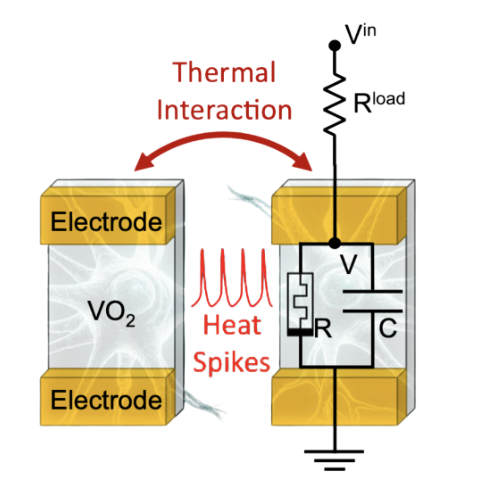
\includegraphics[width=0.92\linewidth]{../vo2_device.png}

\vspace{0.2cm}
{\small Voltage-source equivalent circuit.}
\end{column}
\end{columns}

\slidesource{Starting point: Y.-H. Zhang et al., Nature Communications (2024).}
\note{Explain the competition: the load charges the capacitor, while the VO2 path discharges it. The resistance is not fixed; it is controlled by the thermal state.}
\end{frame}

% ------------------------------------------------
% Slide 4 (1:40-2:20)
% ------------------------------------------------
\begin{frame}{The Feedback Mechanism: Thermal Dynamics}

\begin{columns}[T,onlytextwidth]
\begin{column}{0.61\textwidth}

\textbf{Single-neuristor reduction}

\vspace{0.15cm}

\[
C_{th}\frac{dT}{dt}
=
\underbrace{\frac{V^2}{R_{\mathrm{VO_2}}}}_{\text{Joule heating}}
-
\underbrace{S_e(T-T_0)}_{\text{cooling}}
+
\underbrace{\sigma\eta(t)}_{\text{optional noise}}
\]

\vspace{0.2cm}

\begin{itemize}
    \item \(C_{th}\): thermal inertia of the active device.
    \item \(S_e\): thermal conductance to substrate/environment.
    \item Heating lowers \(R_{\mathrm{VO_2}}\); lower resistance changes the voltage and power.
    \item This delayed negative feedback enables relaxation oscillations.
\end{itemize}

\end{column}

\begin{column}{0.34\textwidth}
\begin{block}{Two coupled state variables}
\[
V(t),\qquad T(t)
\]
\end{block}

\begin{block}{Material memory}
\[
\mathcal H=
\{\delta,T_r,g_r,T_{pr},\ldots\}
\]
\end{block}

\begin{center}
\small
Electrical storage\\
\(\Updownarrow\)\\
Joule heating\\
\(\Updownarrow\)\\
Hysteretic switching
\end{center}
\end{column}
\end{columns}

\slidesource{For one isolated device, the inter-neuristor thermal coupling term is zero.}
\note{Keep this physical: electrical and thermal storage provide two timescales. Hysteresis supplies distinct heating and cooling thresholds.}
\end{frame}

% ------------------------------------------------
% Slide 5 (2:20-3:05)
% ------------------------------------------------
\begin{frame}{Measured Hysteretic Resistance}

\begin{columns}[T,onlytextwidth]
\begin{column}{0.42\textwidth}
\small

\[
R(T,\mathcal H)
=
R_0 e^{(E_a/k_B)/T}
\underbrace{g(T,\mathcal H)}_{\text{insulating fraction}}
+R_m
\]

\[
g=
\frac{1}{2}
+\frac{1}{2}\tanh
\left[
\beta\left(
\delta\frac{w}{2}+T_c-(T+T_p)
\right)
\right]
\]

\scriptsize
\begin{itemize}
    \setlength\itemsep{0.06cm}
    \item \(T_c,w,\beta\): center, width, and steepness.
    \item \(\delta\): heating or cooling direction.
    \item \(T_p\): minor-loop shift after a reversal.
    \item The same law is used in both source configurations.
\end{itemize}

\end{column}

\begin{column}{0.56\textwidth}
\centering
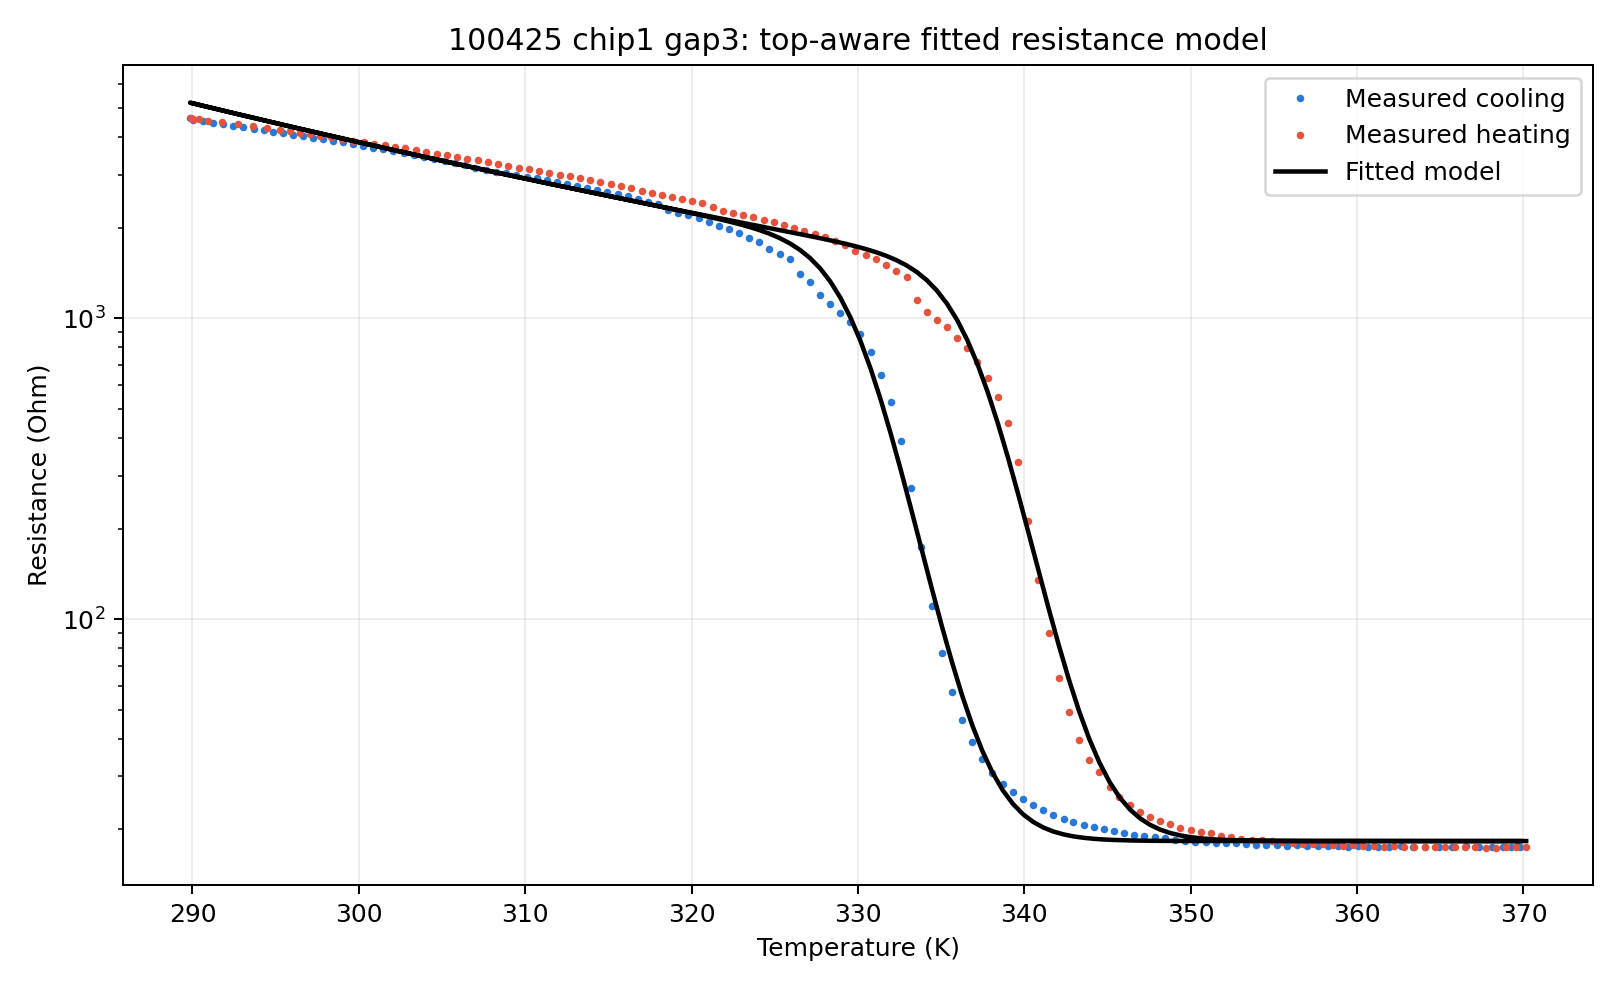
\includegraphics[width=0.91\linewidth]{resistance_fit.png}

\vspace{0.1cm}
{\scriptsize Sample 100425 chip1 gap3; log-space \(R^2\approx0.9987\).}
\end{column}
\end{columns}

\slidesource{Hysteresis: L. A. L. de Almeida et al., Optical Engineering (2002).}
\note{Point out that fitting in log resistance is essential because the transition spans orders of magnitude. The metallic floor is about 18.3 ohm for this sample.}
\end{frame}

% ------------------------------------------------
% Slide 6 (3:05-3:50)
% ------------------------------------------------
\begin{frame}{What Happens at Every Timestep?}

\begin{columns}[T,onlytextwidth]
\begin{column}{0.50\textwidth}
\small

\[
R_n=R(T_n,\mathcal H_n)
\]

\[
V_{n+1}=V_n+\frac{\Delta t}{C}
\left(I_{\mathrm{src},n}-\frac{V_n}{R_n}\right)
\]

\[
T_{n+1}=T_n+\frac{\Delta t}{C_{th}}
\left[
\frac{V_n^2}{R_n}-S_e(T_n-T_0)
\right]
+\frac{\sigma}{C_{th}}\sqrt{\Delta t}\,\zeta_n
\]

\[
I_{\mathrm{src},n}=
\begin{cases}
(V_{in,n}-V_n)/R_{series}, & \text{voltage drive},\\
I_{in,n}, & \text{current drive}.
\end{cases}
\]

\end{column}

\begin{column}{0.47\textwidth}
\centering
\begin{tikzpicture}[node distance=0.30cm]
    \node[flowbox] (r) {1. Evaluate \(R_n\) from \(T_n,\mathcal H_n\)};
    \node[flowbox, below=of r] (v) {2. Update electrical state \(V_{n+1}\)};
    \node[flowbox, below=of v] (p) {3. Compute \(P_n=V_n^2/R_n\)};
    \node[flowbox, below=of p] (t) {4. Update thermal state \(T_{n+1}\)};
    \node[flowbox, below=of t] (h) {5. Update reversal memory \(\mathcal H_{n+1}\)};
    \draw[flowarrow] (r) -- (v);
    \draw[flowarrow] (v) -- (p);
    \draw[flowarrow] (p) -- (t);
    \draw[flowarrow] (t) -- (h);
    \draw[flowarrow] (h.east) -- ++(0.65,0) |- (r.east);
\end{tikzpicture}

\vspace{0.12cm}
{\scriptsize Forward Euler; Euler--Maruyama when \(\sigma>0\).\\
Production sweeps use \(\sigma=0\).}
\end{column}
\end{columns}

\note{This slide replaces the long derivation. Stress the update order: resistance is evaluated from the current thermal state, then electrical and thermal states advance, then hysteresis memory is updated.}
\end{frame}

% ------------------------------------------------
% Slide 7 (3:50-4:35)
% ------------------------------------------------
\begin{frame}{From Voltage Drive to Ideal Current Drive}

\begin{columns}[T,onlytextwidth]
\begin{column}{0.47\textwidth}
\begin{block}{Original voltage source}
\[
C\frac{dV}{dt}
=
\frac{V_{in}-V}{R_{series}}
-\frac{V}{R}
\]
\[
I_{\mathrm{src}} \text{ changes with } V
\]
\end{block}
\end{column}

\begin{column}{0.47\textwidth}
\begin{alertblock}{Ideal imposed current}
\[
I_{in}=C\frac{dV}{dt}+\frac{V}{R}
\]
\[
\boxed{
C\frac{dV}{dt}=I_{in}-\frac{V}{R}
}
\]
\end{alertblock}
\end{column}
\end{columns}

\vspace{0.2cm}

\begin{center}
\begin{tabular}{ll}
\toprule
\textbf{Preserved} & \textbf{Assumed in the current-source reduction} \\
\midrule
Yuanhang \(R(T,\mathcal H)\) & one VO\textsubscript{2} device/domain \\
single thermal state \(T\) & one thermal node \\
Joule heating and cooling & ideal imposed current \\
optional stochastic heating & no added phase-lag state \\
\bottomrule
\end{tabular}
\end{center}

\vspace{0.12cm}
\begin{center}
\alert{\textbf{The circuit boundary condition changed; the material mathematics did not.}}
\end{center}

\note{Derive the current equation directly from KCL. This is the clean answer to whether we changed the mathematics: the hysteresis law is unchanged; only the source boundary condition differs.}
\end{frame}

% ------------------------------------------------
% Slide 8 (4:35-5:15)
% ------------------------------------------------
\begin{frame}{New Problem: The Oscillatory Domain Was Unknown}

\begin{columns}[T,onlytextwidth]
\begin{column}{0.48\textwidth}
\begin{block}{Physical controls}
\begin{tabular}{ll}
\(I_{in}\) & imposed electrical drive \\
\(C\) & electrical charging time \\
\(C_{th}\) & thermal inertia \\
\(S_e\) & environmental cooling \\
\(T_0\) & starting/ambient temperature \\
\end{tabular}
\end{block}

\[
\tau_e\sim R C,
\qquad
\tau_{th}\sim \frac{C_{th}}{S_e}
\]

\small
Oscillations require enough Joule heating to cross the transition, but enough
cooling and electrical recovery to return.
\end{column}

\begin{column}{0.48\textwidth}
\begin{alertblock}{Acceptance criteria}
\begin{enumerate}
    \item Oscillations persist in a late-time window.
    \item More than one full cycle is present.
    \item Startup overshoot is excluded.
    \item Frequency is below the numerical/Nyquist limit.
    \item Period and amplitude survive timestep refinement.
    \item The path is interpretable on \(R(T,\mathcal H)\).
\end{enumerate}
\end{alertblock}
\end{column}
\end{columns}

\note{Explain why a blind sweep is not enough. A classifier can call overshoot an oscillation, so the scientific definition must include late-time persistence and convergence.}
\end{frame}

% ------------------------------------------------
% Slide 9 (5:15-5:55)
% ------------------------------------------------
\begin{frame}{How I Used Codex as a Research Tool}

\begin{center}
\begin{tikzpicture}[node distance=0.30cm]
    \node[flowbox, text width=2.0cm] (constraint) {\textbf{Constrain}\\use existing equations and APIs};
    \node[flowbox, right=of constraint, text width=2.0cm] (sweep) {\textbf{Sweep}\\physical parameter ranges};
    \node[flowbox, right=of sweep, text width=2.0cm] (classify) {\textbf{Classify}\\late-window traces};
    \node[flowbox, right=of classify, text width=2.0cm] (verify) {\textbf{Verify}\\timestep and duration};
    \node[flowbox, right=of verify, text width=2.0cm] (save) {\textbf{Record}\\plots, CSV, app History};
    \draw[flowarrow] (constraint) -- (sweep);
    \draw[flowarrow] (sweep) -- (classify);
    \draw[flowarrow] (classify) -- (verify);
    \draw[flowarrow] (verify) -- (save);
\end{tikzpicture}
\end{center}

\vspace{0.25cm}

\begin{block}{Representative instruction}
\small
``Use the existing current-source simulator without changing the model. Sweep
physical values of current, capacitance, thermal capacitance, and thermal
conductance. Find sustained oscillations, reject startup overshoot and numerical
artifacts, and save successful simulations into app History.''
\end{block}

\begin{columns}[T,onlytextwidth]
\begin{column}{0.47\textwidth}
\textbf{Codex accelerated}
\begin{itemize}
    \item search-script implementation;
    \item repeated simulations and plots;
    \item trace metrics and job registration.
\end{itemize}
\end{column}
\begin{column}{0.47\textwidth}
\textbf{Scientific control remained}
\begin{itemize}
    \item equations and physical constraints;
    \item acceptance/rejection criteria;
    \item interpretation and final claims.
\end{itemize}
\end{column}
\end{columns}

\note{Do not present AI as producing the scientific answer. Present it as a repository-integrated computational assistant that made a constrained, reproducible search practical.}
\end{frame}

% ------------------------------------------------
% Slide 10 (5:55-6:45)
% ------------------------------------------------
\begin{frame}{Result: Three Current-Driven Regimes}
\centering

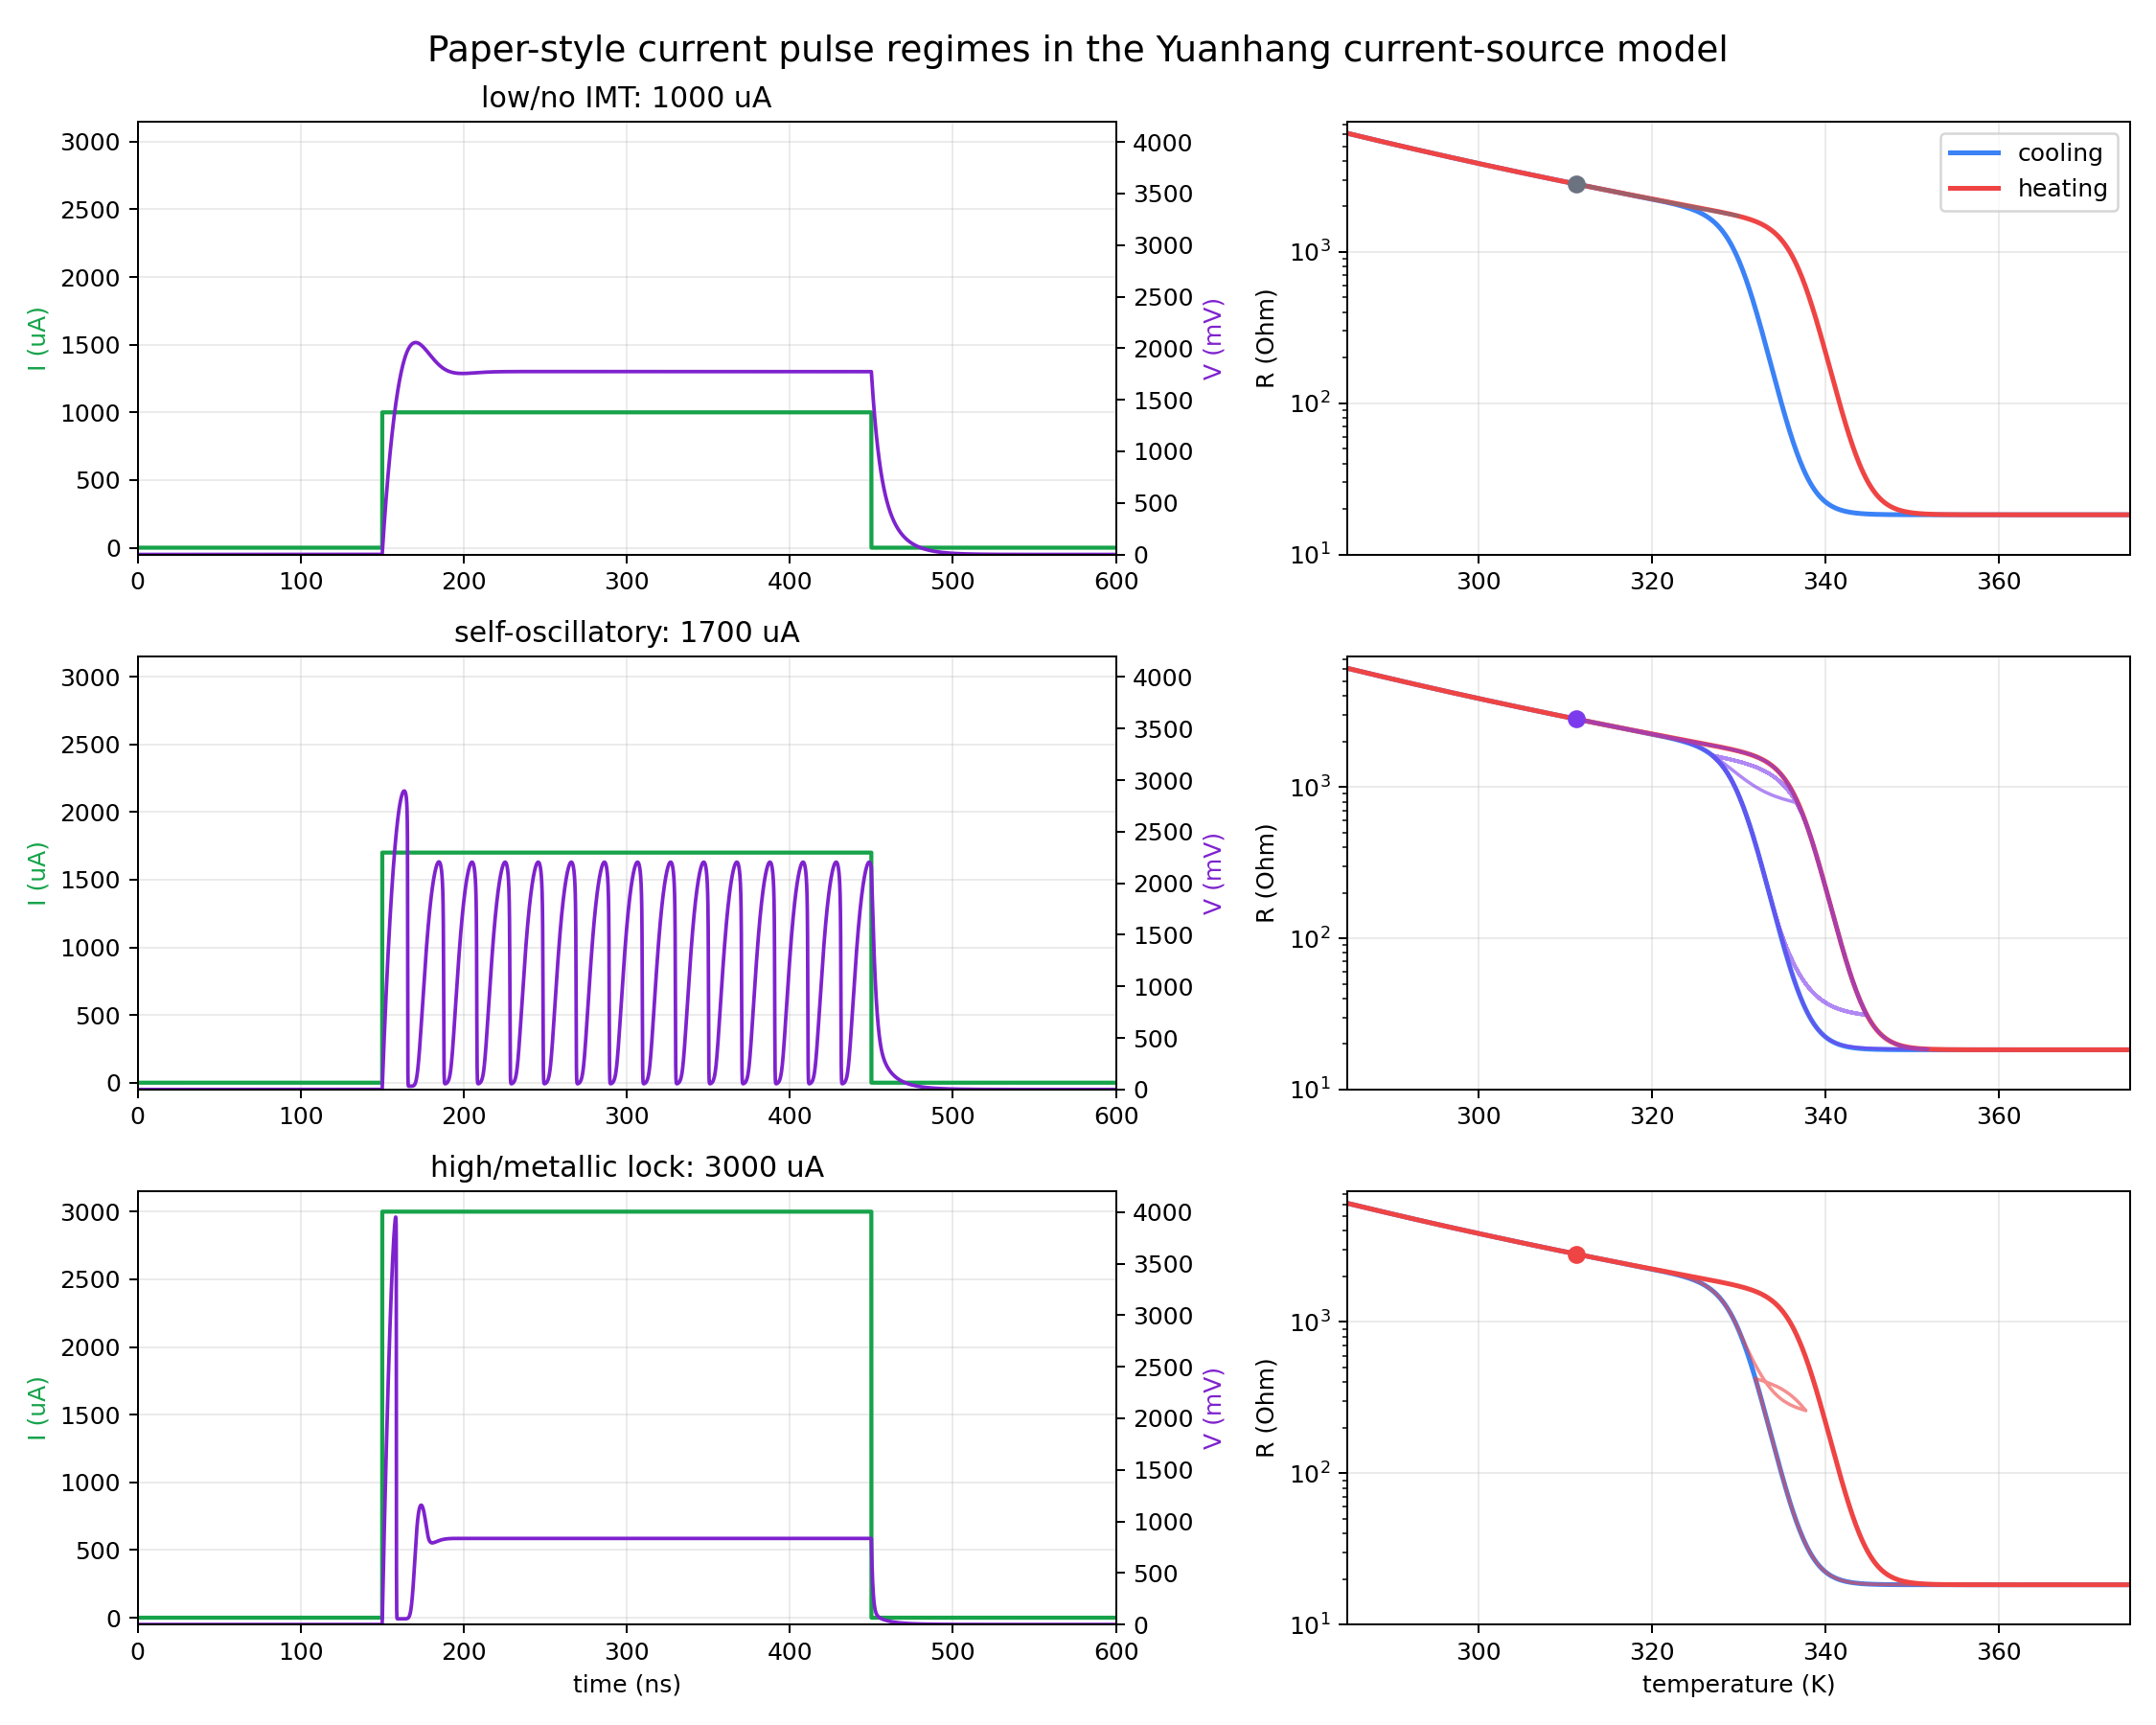
\includegraphics[height=0.77\textheight]{three_regimes.png}

\vspace{0.04cm}
{\scriptsize
Low current: insulating equilibrium \(\rightarrow\)
intermediate current: relaxation oscillation \(\rightarrow\)
high current: metallic lock.
}

\note{Walk down the rows. At low current the device never reaches the transition. In the middle it repeatedly traverses a minor hysteresis loop. At high current it cannot cool back, so it locks metallic.}
\end{frame}

% ------------------------------------------------
% Slide 11 (6:45-7:30)
% ------------------------------------------------
\begin{frame}{What the Simulation Reveals Inside One Oscillation}
\centering

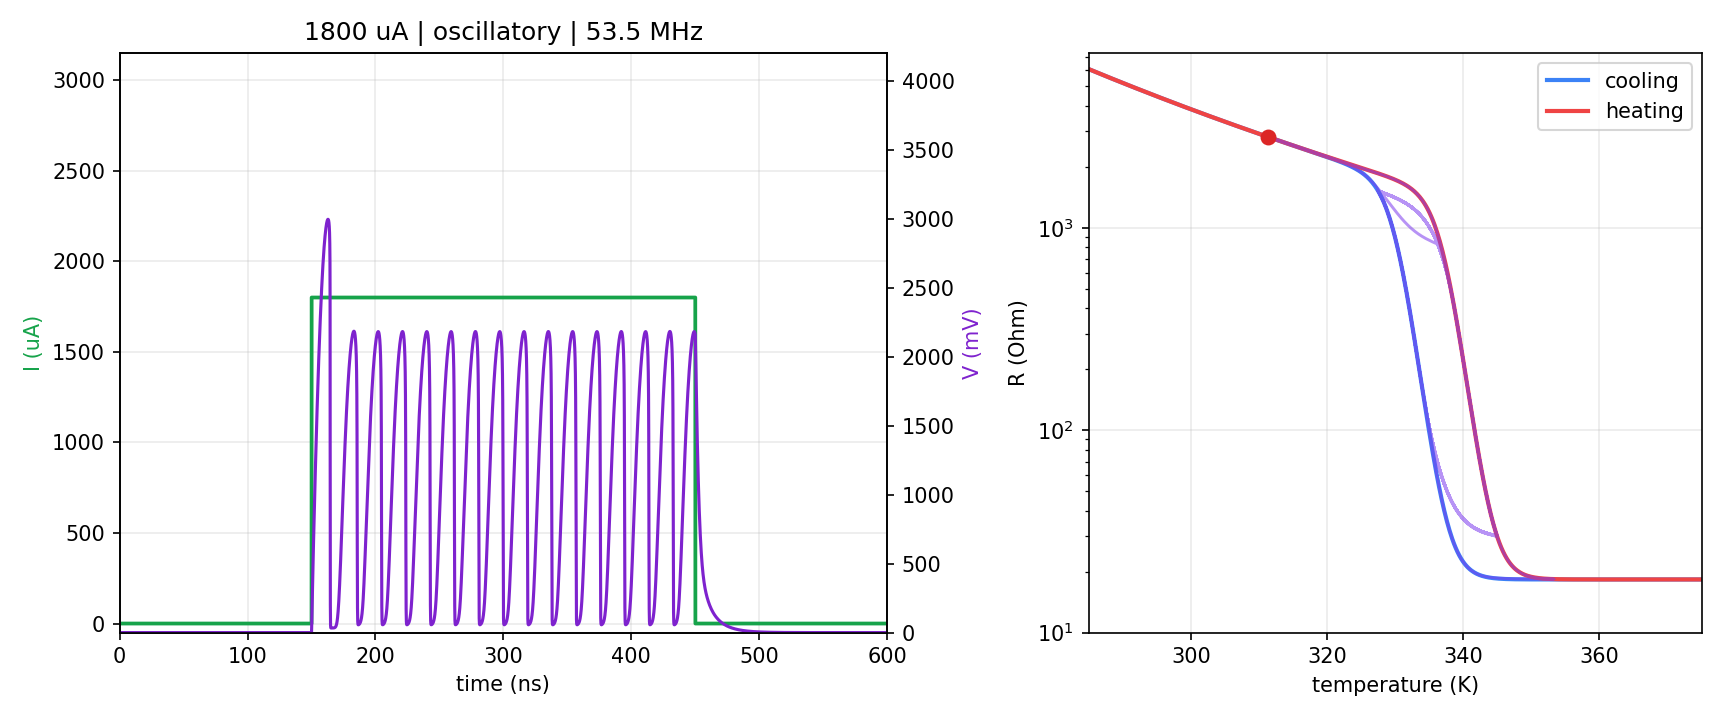
\includegraphics[width=0.92\linewidth]{oscillation_1800uA.png}

\vspace{0.05cm}
{\scriptsize
\(\SI{1800}{\micro\ampere}\): sustained \(\SI{53.5}{\mega\hertz}\) voltage
oscillation. The right panel exposes the otherwise hidden trajectory through the
hysteresis loop.
}

\vspace{0.05cm}
\href{run:media/paper_frequency_1800uA_time_evolution_10s.gif}{
\beamergotobutton{Open 10-second time-evolution animation}
}

\note{Use the left panel for what the oscilloscope sees and the right panel for what the simulator adds. The trajectory is the physical explanation: heat, switch, discharge, cool, recover, repeat.}
\end{frame}

% ------------------------------------------------
% Slide 12 (7:30-8:05)
% ------------------------------------------------
\begin{frame}{Higher-Frequency Oscillation: \(\SI{57.1}{\mega\hertz}\)}
\centering

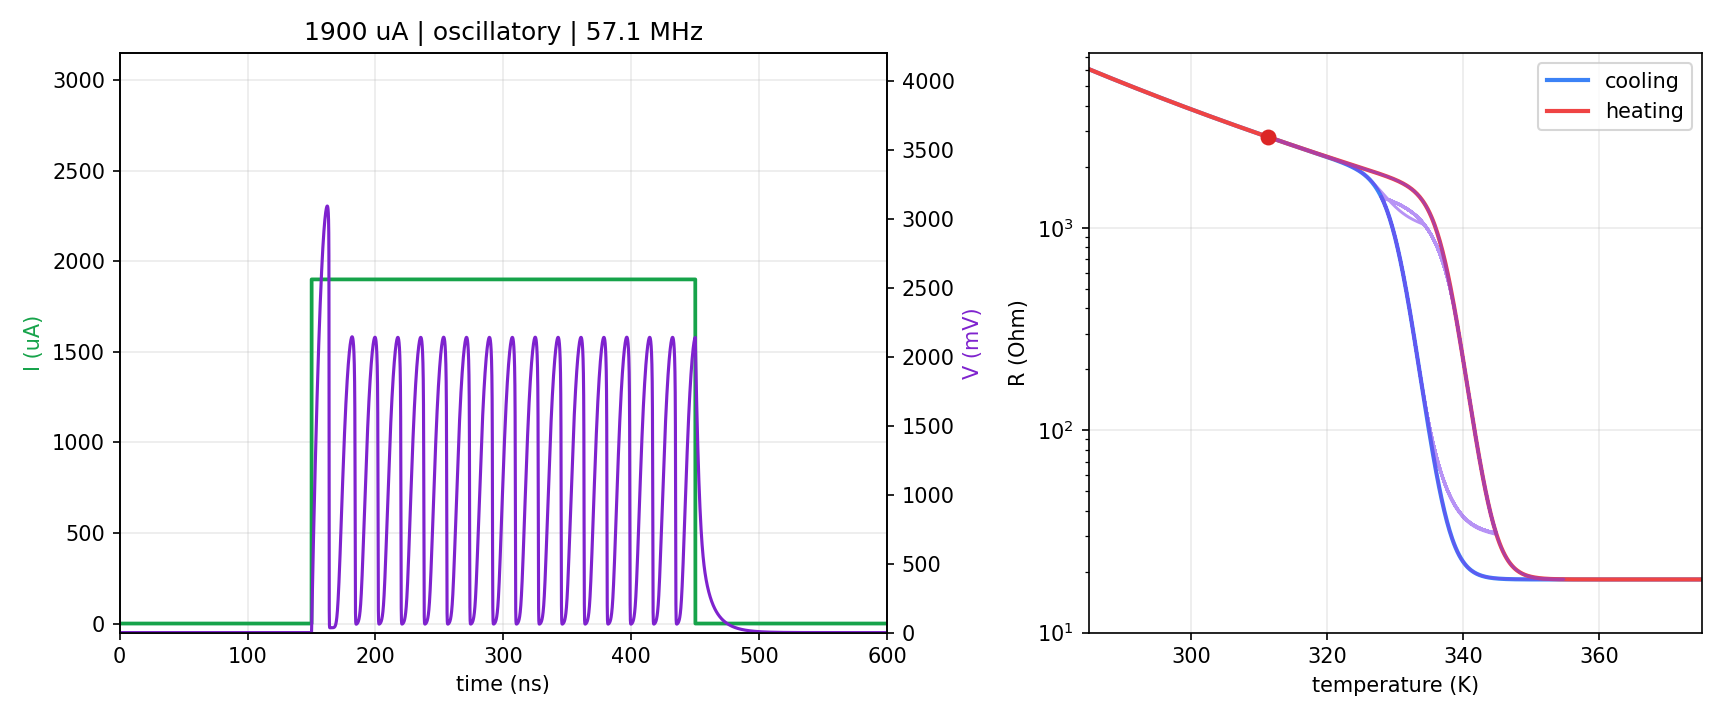
\includegraphics[width=0.93\linewidth]{high_frequency_1900uA.png}

\vspace{0.04cm}
{\scriptsize
\(\SI{1900}{\micro\ampere}\),
\(C=\SI{4}{\pico\farad}\),
\(C_{th}=\SI{1}{\pico\joule\per\kelvin}\):
\(\SI{57.1}{\mega\hertz}\), \(V_{pp}\approx\SI{2.08}{\volt}\), and
\(E_{\mathrm{cycle}}\approx\SI{39.1}{\pico\joule}\).
The trajectory repeatedly closes a stable minor loop.
}

\vspace{0.05cm}
\href{run:media/paper_frequency_current_sweep.gif}{
\beamergotobutton{Open high-frequency current-sweep animation}
}

\note{This is a higher-current point in the paper-frequency parameter set. Compared with 1800 microamperes, the cycle is faster, the amplitude is slightly smaller, and the hysteresis path remains stable.}
\end{frame}

% ------------------------------------------------
% Slide 13 (8:05-8:40)
% ------------------------------------------------
\begin{frame}{Upper Edge of the Oscillatory Window}
\centering

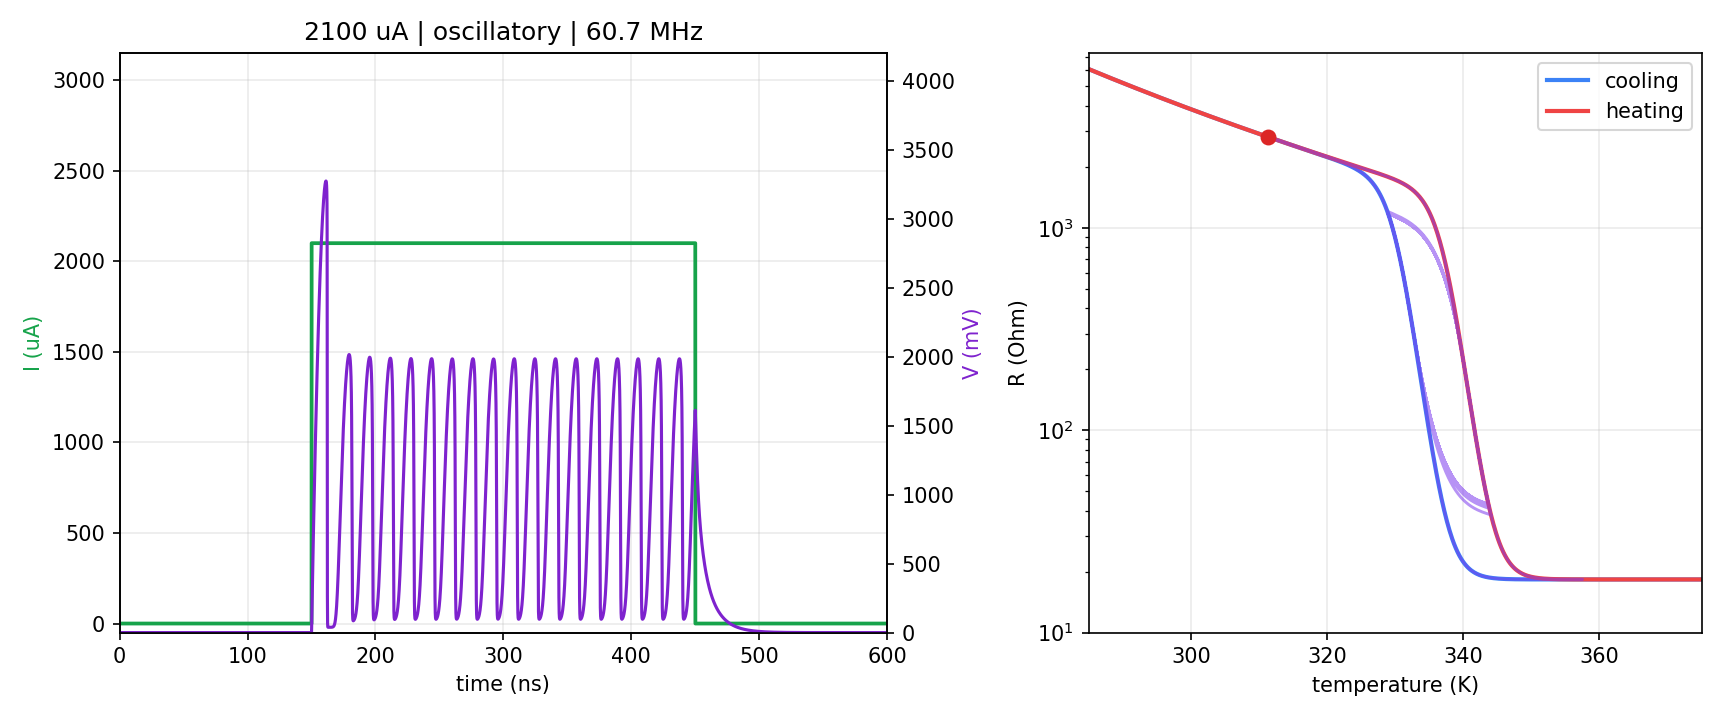
\includegraphics[width=0.94\linewidth]{high_frequency_2100uA.png}

\vspace{0.04cm}
{\scriptsize
At \(\SI{2100}{\micro\ampere}\), frequency reaches
\(\SI{60.7}{\mega\hertz}\), \(V_{pp}\approx\SI{1.89}{\volt}\), and
\(E_{\mathrm{cycle}}\approx\SI{36.3}{\pico\joule}\).
This is the last sustained point before metallic lock at
\(\SI{2200}{\micro\ampere}\).
}

\note{This operating point marks the high-frequency edge of the domain. Increasing current further prevents sufficient cooling and the device settles into the metallic-lock regime instead of completing another relaxation cycle.}
\end{frame}

% ------------------------------------------------
% Slide 14 (8:40-9:10)
% ------------------------------------------------
\begin{frame}{Mapped Operating Window}

\centering
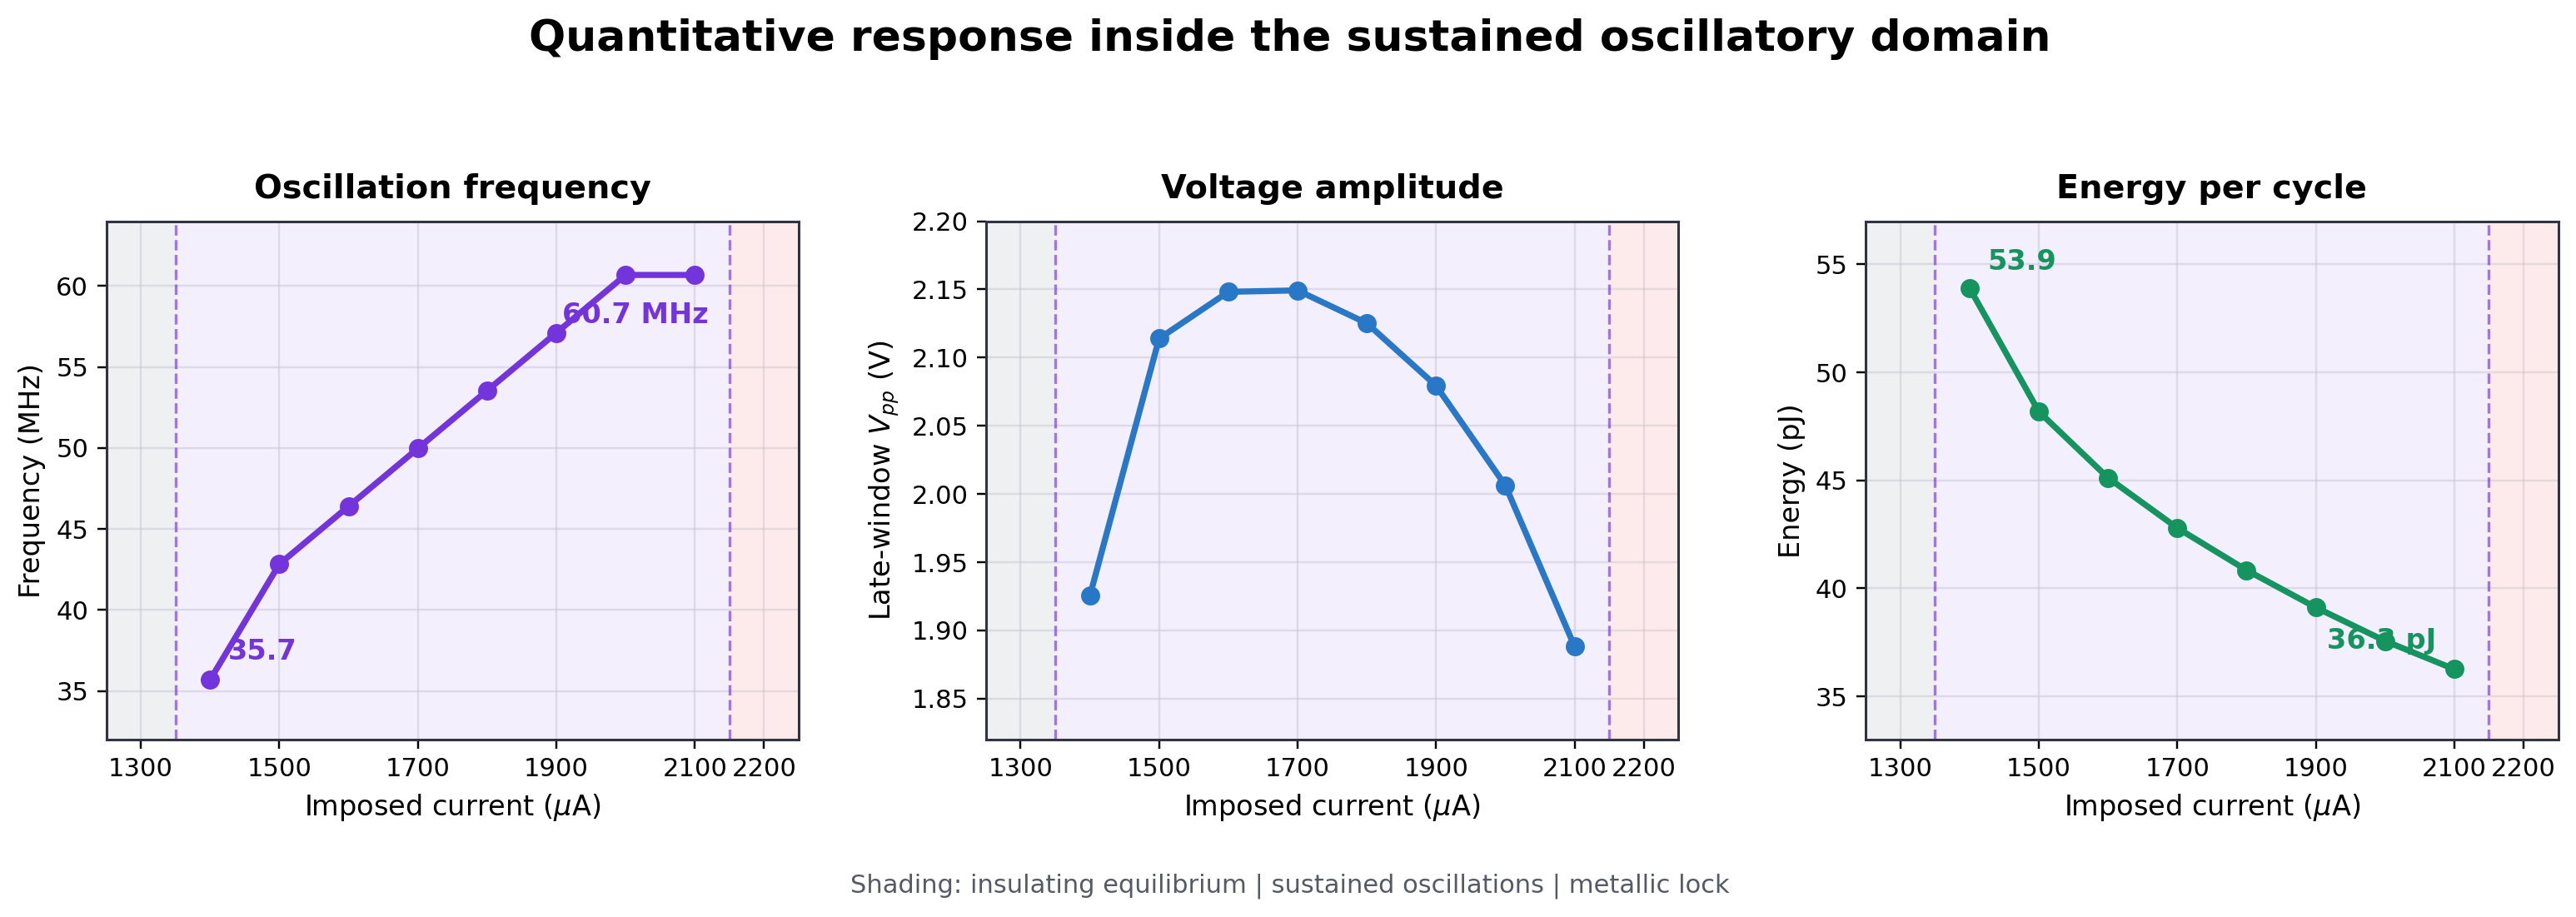
\includegraphics[width=0.97\linewidth]{operating_window_response.png}

\vspace{0.08cm}

\small
\textbf{Window:} \(\SIrange{1400}{2100}{\micro\ampere}\).
Frequency increases while cycle energy decreases; voltage amplitude remains
approximately \(\SI{2}{\volt}\).

\vspace{0.04cm}
{\scriptsize
\(C=\SI{4}{\pico\farad}\), \(C_{th}=\SI{1}{\pico\joule\per\kelvin}\),
\(S_e=\SI{0.10}{\milli\watt\per\kelvin}\); current applied from
\(\SI{150}{\nano\second}\) to \(\SI{450}{\nano\second}\).
}

\note{The key result is a contiguous domain, not one lucky trace. Frequency rises through the oscillatory band, and the system exits into metallic lock at higher current.}
\end{frame}

% ------------------------------------------------
% Slide 15 (9:10-9:35)
% ------------------------------------------------
\begin{frame}{What Is Established, and What Is Not}

\begin{columns}[T,onlytextwidth]
\begin{column}{0.48\textwidth}
\begin{block}{Supported by the simulations}
\begin{itemize}
    \item The original Yuanhang hysteresis mechanism can oscillate under ideal current drive.
    \item Low, oscillatory, and metallic-lock regimes emerge without adding a phase-delay state.
    \item The paper-frequency analog reaches \(\SIrange{35.7}{60.7}{\mega\hertz}\).
    \item Serial and vectorized traces agree; representative periods converge with smaller \(\Delta t\).
\end{itemize}
\end{block}
\end{column}

\begin{column}{0.48\textwidth}
\begin{alertblock}{Not yet an absolute experimental fit}
\begin{itemize}
    \item The simulated current window is higher than the measured one.
    \item Cycle energy is \(\sim\SIrange{36}{54}{\pico\joule}\), not the paper's \(\sim\SIrange{1}{2}{\pico\joule}\).
    \item \(C\), \(C_{th}\), \(S_e\), and source non-ideality need transient calibration.
    \item The model is phenomenologically corroborative, not parameter-identical.
\end{itemize}
\end{alertblock}
\end{column}
\end{columns}

\note{This slide protects the scientific claim. We reproduce the mechanism, regime sequence, and frequency scale, but we should not claim a full quantitative fit to current or energy yet.}
\end{frame}

% ------------------------------------------------
% Slide 16: transition from the July mechanism study to specimen calibration
% ------------------------------------------------
\begin{frame}{From Mechanism Demonstration to Specimen Calibration}

\begin{columns}[T,onlytextwidth]
\begin{column}{0.37\textwidth}
\begin{block}{What the July study established}
\small
The preserved Yuanhang hysteresis mechanism can generate robust
current-driven relaxation oscillations in a verified numerical domain.
\end{block}

\begin{alertblock}{What it did not establish}
\small
The illustrative parameter set did not reproduce the measured current window,
voltage amplitude, or energy scale.
\end{alertblock}
\end{column}

\begin{column}{0.59\textwidth}
\textbf{Specimen-specific inference chain}

\vspace{0.20cm}
\begin{tikzpicture}[node distance=0.23cm]
    \node[flowbox, text width=2.05cm] (input) {Measured input\\\(I(t)\), pulse timing};
    \node[flowbox, right=of input, text width=2.05cm] (static) {Static conditions\\\(T_0\), \(R(T)\), \(\gamma\)};
    \node[flowbox, right=of static, text width=2.05cm] (thermal) {Dynamic estimates\\\(S_e\), \(C\), \(C_{th}\)};
    \draw[flowarrow] (input) -- (static);
    \draw[flowarrow] (static) -- (thermal);
\end{tikzpicture}

\vspace{0.25cm}
\begin{enumerate}
    \item Estimate each quantity from the most direct available evidence.
    \item Record whether it is fitted, adopted, bounded, or borrowed.
    \item Freeze one parameter vector before replaying the full current sweep.
\end{enumerate}
\end{column}
\end{columns}

\slidesource{Numerical evidence: reviewed bundles in \texttt{public\_jobs/}; no per-trace tuning in the final replay.}
\note{This slide connects the original mechanism talk to the specimen-calibration work. The key methodological rule is to estimate each quantity once, record its evidence status, and only then compare against all measured traces.}
\end{frame}

% ------------------------------------------------
% Slide 17: measured input current
% ------------------------------------------------
\begin{frame}{Input Current \(I(t)\): Replay the Measured Waveform}
\centering

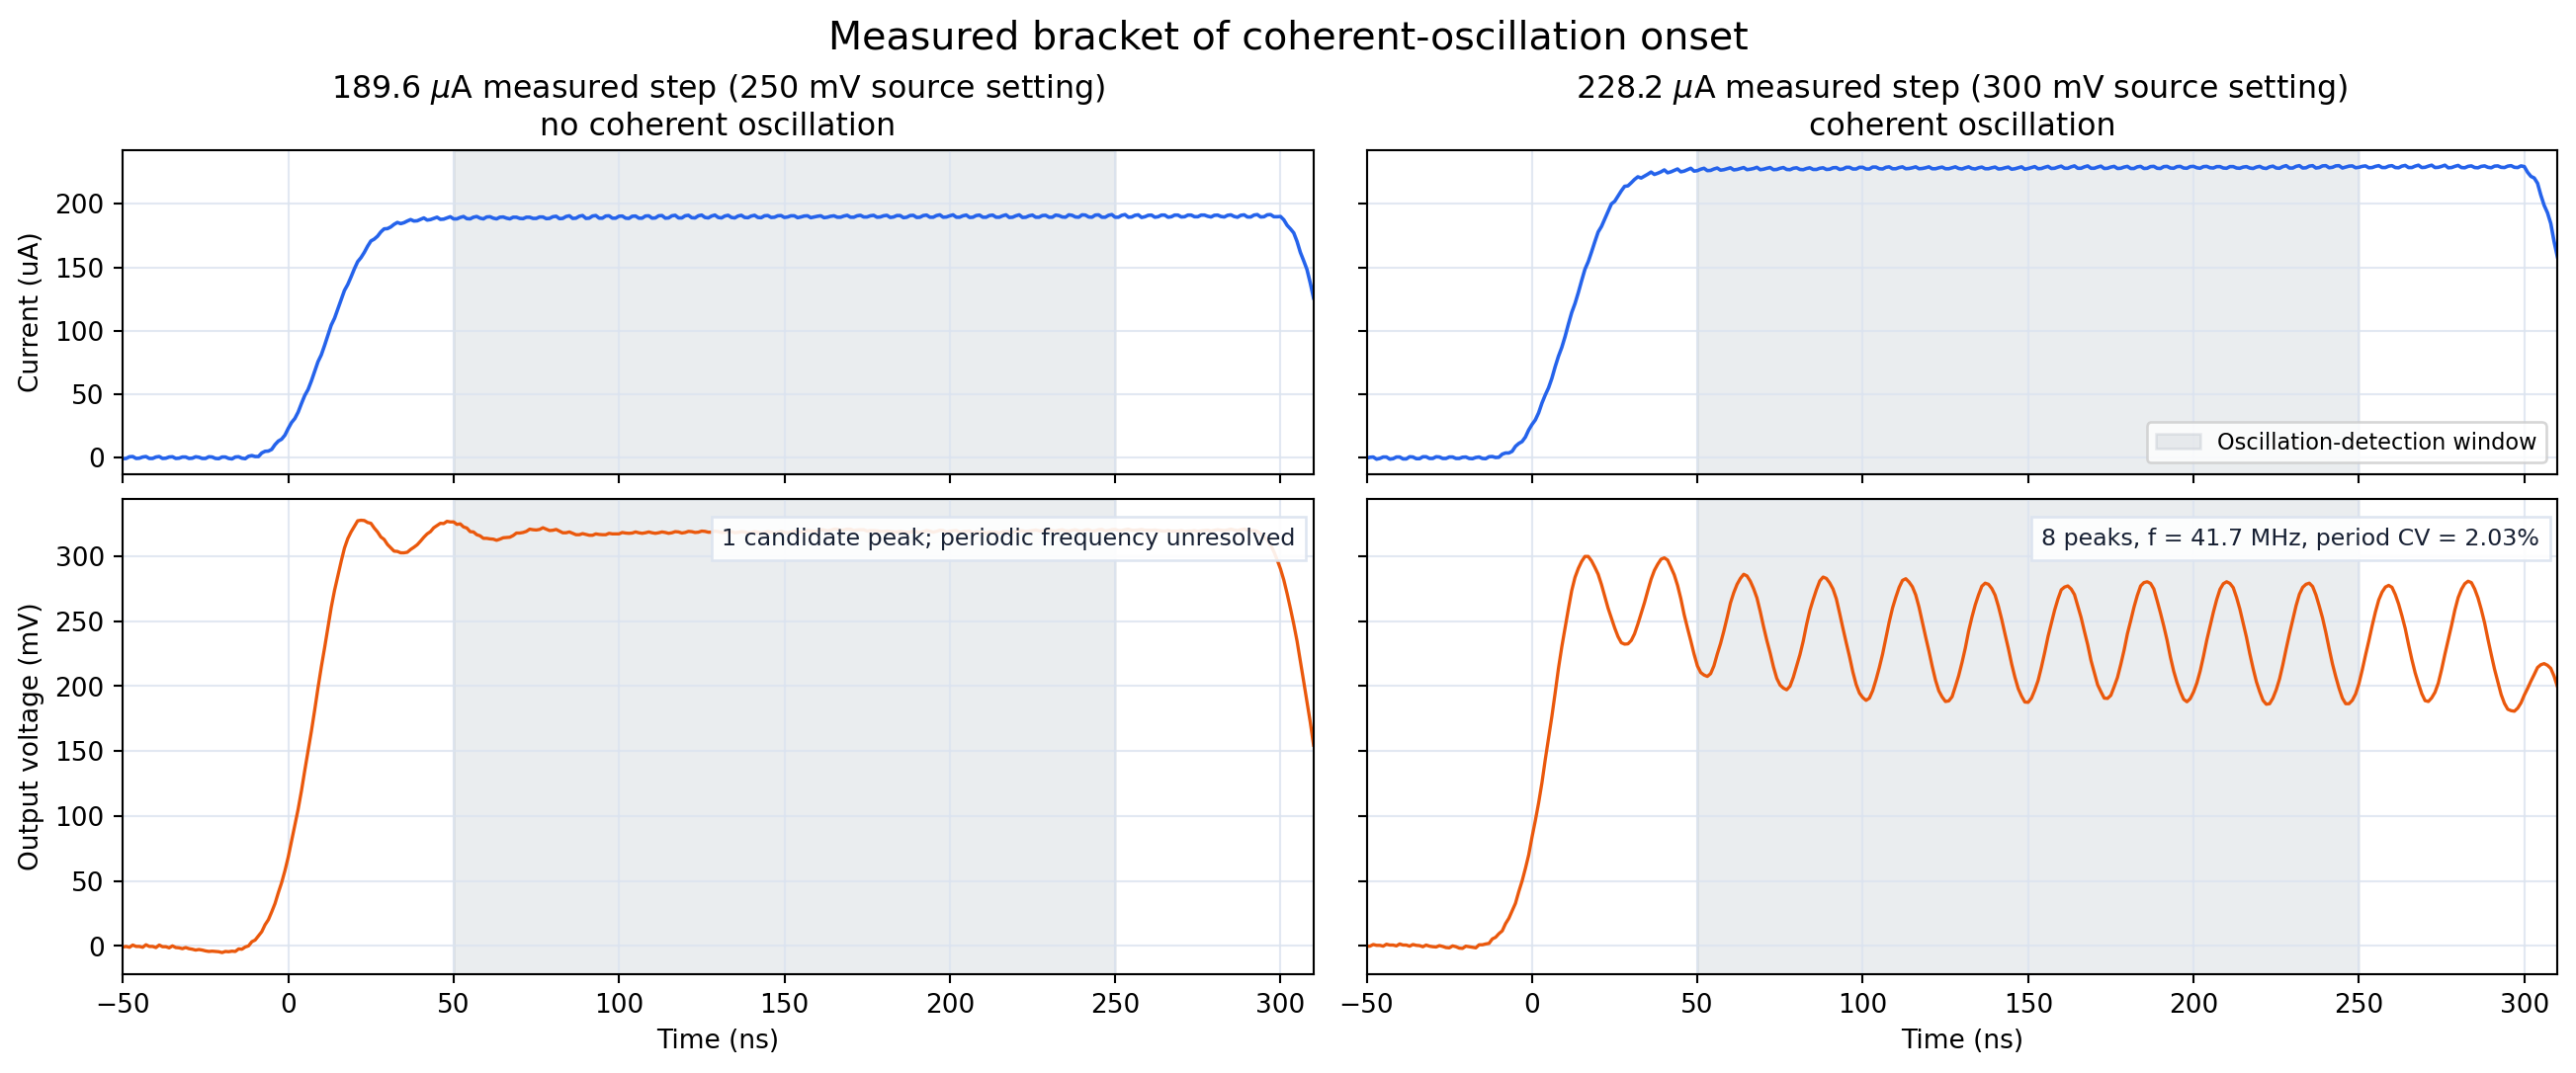
\includegraphics[height=0.58\textheight]{../public_jobs/20260827_142103_measured-laboratory-current-sweep-with-current-l_ec6ec4/figures/oscillation_onset_bracket.png}

\vspace{0.08cm}
\begin{columns}[T,onlytextwidth]
\begin{column}{0.47\textwidth}
\small
\textbf{Measured operating input}
\[
I_{\mathrm{model}}(t)=I_{\mathrm{measured}}(t)
\]
\end{column}
\begin{column}{0.50\textwidth}
\scriptsize
The 250 and 300 mV source settings correspond to measured current steps of
\(189.6\) and \(228.2~\mu\mathrm{A}\). The pulse lasts \(300\) ns, with a
26--27 ns rise and an 18--23 ns fall.
\end{column}
\end{columns}

\slidesource{Professor-supplied numerical traces; archived onset analysis \texttt{ec6ec4}.}
\note{The filename voltage is only a source-setting label. The model input is the measured current waveform, including the non-instantaneous edge. The two adjacent records provide a measured onset bracket.}
\end{frame}

% ------------------------------------------------
% Slide 18: ambient temperature
% ------------------------------------------------
\begin{frame}{Ambient Temperature \(T_0\): Adopted Experimental Condition}

\begin{columns}[T,onlytextwidth]
\begin{column}{0.53\textwidth}
\begin{block}{Role in the thermal balance}
\[
C_{th}\frac{dT}{dt}=P-S_e(T-T_0)
\]
\[
\Delta T=T-T_0
\]
\end{block}

\small
The TIA sweep did not contain an independent thermometer record. We therefore
adopted the ambient range reported for the related measurements rather than
fitting \(T_0\) from the electrical traces.
\end{column}

\begin{column}{0.43\textwidth}
\begin{alertblock}{Adopted value}
\centering
\Large
\[
\boxed{T_0=314.4~\mathrm{K}}
\]
\normalsize
reported range: 314.25--314.55 K
\end{alertblock}

\vspace{0.30cm}
\begin{center}
\begin{tikzpicture}[x=0.40cm]
    \draw[very thick,structure.fg] (0,0)--(10,0);
    \draw[thick] (0,-0.15)--(0,0.15) node[below=4pt] {\scriptsize 314.25};
    \draw[thick] (5,-0.15)--(5,0.15) node[below=4pt] {\scriptsize 314.40};
    \draw[thick] (10,-0.15)--(10,0.15) node[below=4pt] {\scriptsize 314.55 K};
    \fill[tracered] (5,0) circle (2.2pt);
\end{tikzpicture}
\end{center}
\end{column}
\end{columns}

\vspace{0.25cm}
\begin{alertblock}{Interpretation}
\small
This is an adopted boundary condition, not a specimen-specific fit. Its
applicability to the exact TIA run remains an experimental check.
\end{alertblock}

\slidesource{Ambient range: Gildor et al., arXiv:2604.04594v1; inference status recorded in the research handoff.}
\note{Be explicit about evidence status. T0 enters every thermal estimate through the temperature rise, but it was not inferred from the current-sweep waveforms.}
\end{frame}

% ------------------------------------------------
% Slide 19: major-loop resistance parameters
% ------------------------------------------------
\begin{frame}{Resistance Parameters: Fit the Measured Major Loop}

\begin{columns}[T,onlytextwidth]
\begin{column}{0.38\textwidth}
\scriptsize
\[
\min_{\theta}\sum_i
\left[\log_{10}R_{\mathrm{model}}(T_i;\theta)
-\log_{10}R_i\right]^2
\]

\begin{tabular}{@{}lrr@{}}
\toprule
\textbf{Parameter} & \textbf{Specimen} & \textbf{Yuanhang} \\
\midrule
\(R_0\) (\(\Omega\)) & 0.7989 & 0.00536 \\
\(E_a/k_B\) (K) & 2536.97 & 5220.47 \\
\(R_m\) (\(\Omega\)) & 18.215 & 1286.32 \\
\(T_c\) (K) & 333.494 & 332.806 \\
\(w\) (K) & 6.882 & 7.194 \\
\(\beta\) (K\(^{-1}\)) & 0.2992 & 0.2528 \\
\bottomrule
\end{tabular}

\vspace{0.18cm}
\begin{block}{Fit quality}
\centering
\(R^2=0.99873\)\qquad
\(\mathrm{RMSE}_{\log_{10}R}=0.03663\)
\end{block}
\end{column}

\begin{column}{0.60\textwidth}
\centering
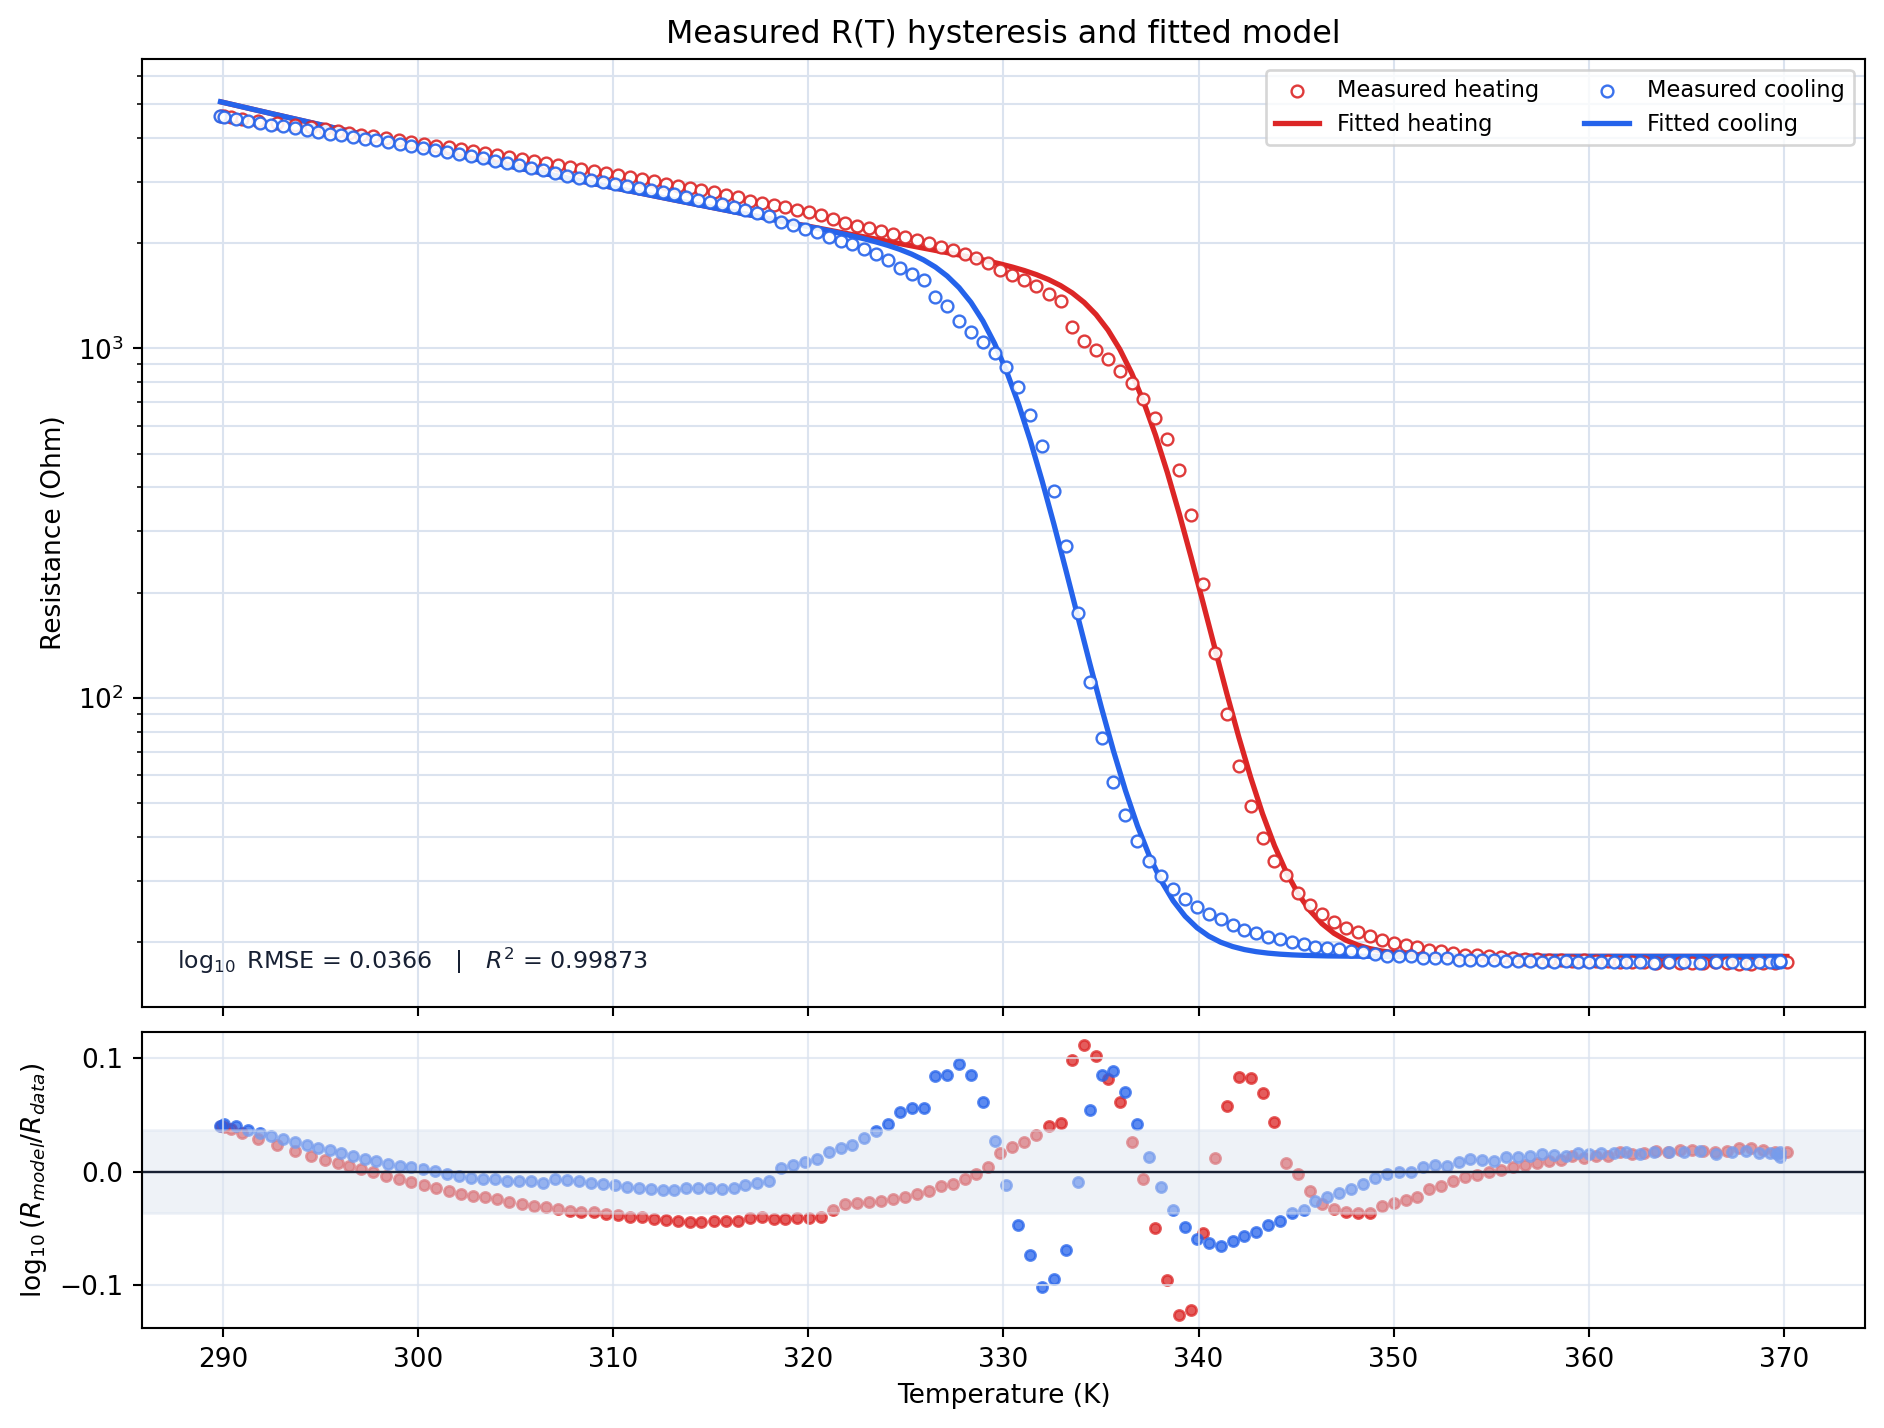
\includegraphics[width=\linewidth]{../public_jobs/20260816_125905_sample-r-t-major-loop-hysteresis-fit_0849a9/figures/resistance_fit.png}
\end{column}
\end{columns}

\slidesource{264 measured points from sample 100425 chip1 gap3; reviewed fit bundle \texttt{0849a9}.}
\note{The logarithmic residual gives comparable weight to both resistance decades. R0 is only the Arrhenius prefactor. The full insulating resistance includes the exponential term, so it remains far above the fitted metallic floor.}
\end{frame}

% ------------------------------------------------
% Slide 20: gamma
% ------------------------------------------------
\begin{frame}{Minor-Loop Memory \(\gamma\): Not Identified by the Major Loop}

\begin{columns}[T,onlytextwidth]
\begin{column}{0.43\textwidth}
\small
\begin{block}{What the measurement determines}
One complete heating branch and one complete cooling branch constrain
\(R_0,E_a,R_m,T_c,w\), and \(\beta\).
\end{block}

\begin{alertblock}{What \(\gamma\) controls}
\(\gamma\) changes the reversal-dependent minor-loop return. A single major loop
contains no independent family of partial reversals, so it cannot determine
\(\gamma\).
\end{alertblock}

\[
\boxed{\gamma=0.95627\ \text{(borrowed from Yuanhang)}}
\]

\end{column}

\begin{column}{0.55\textwidth}
\centering
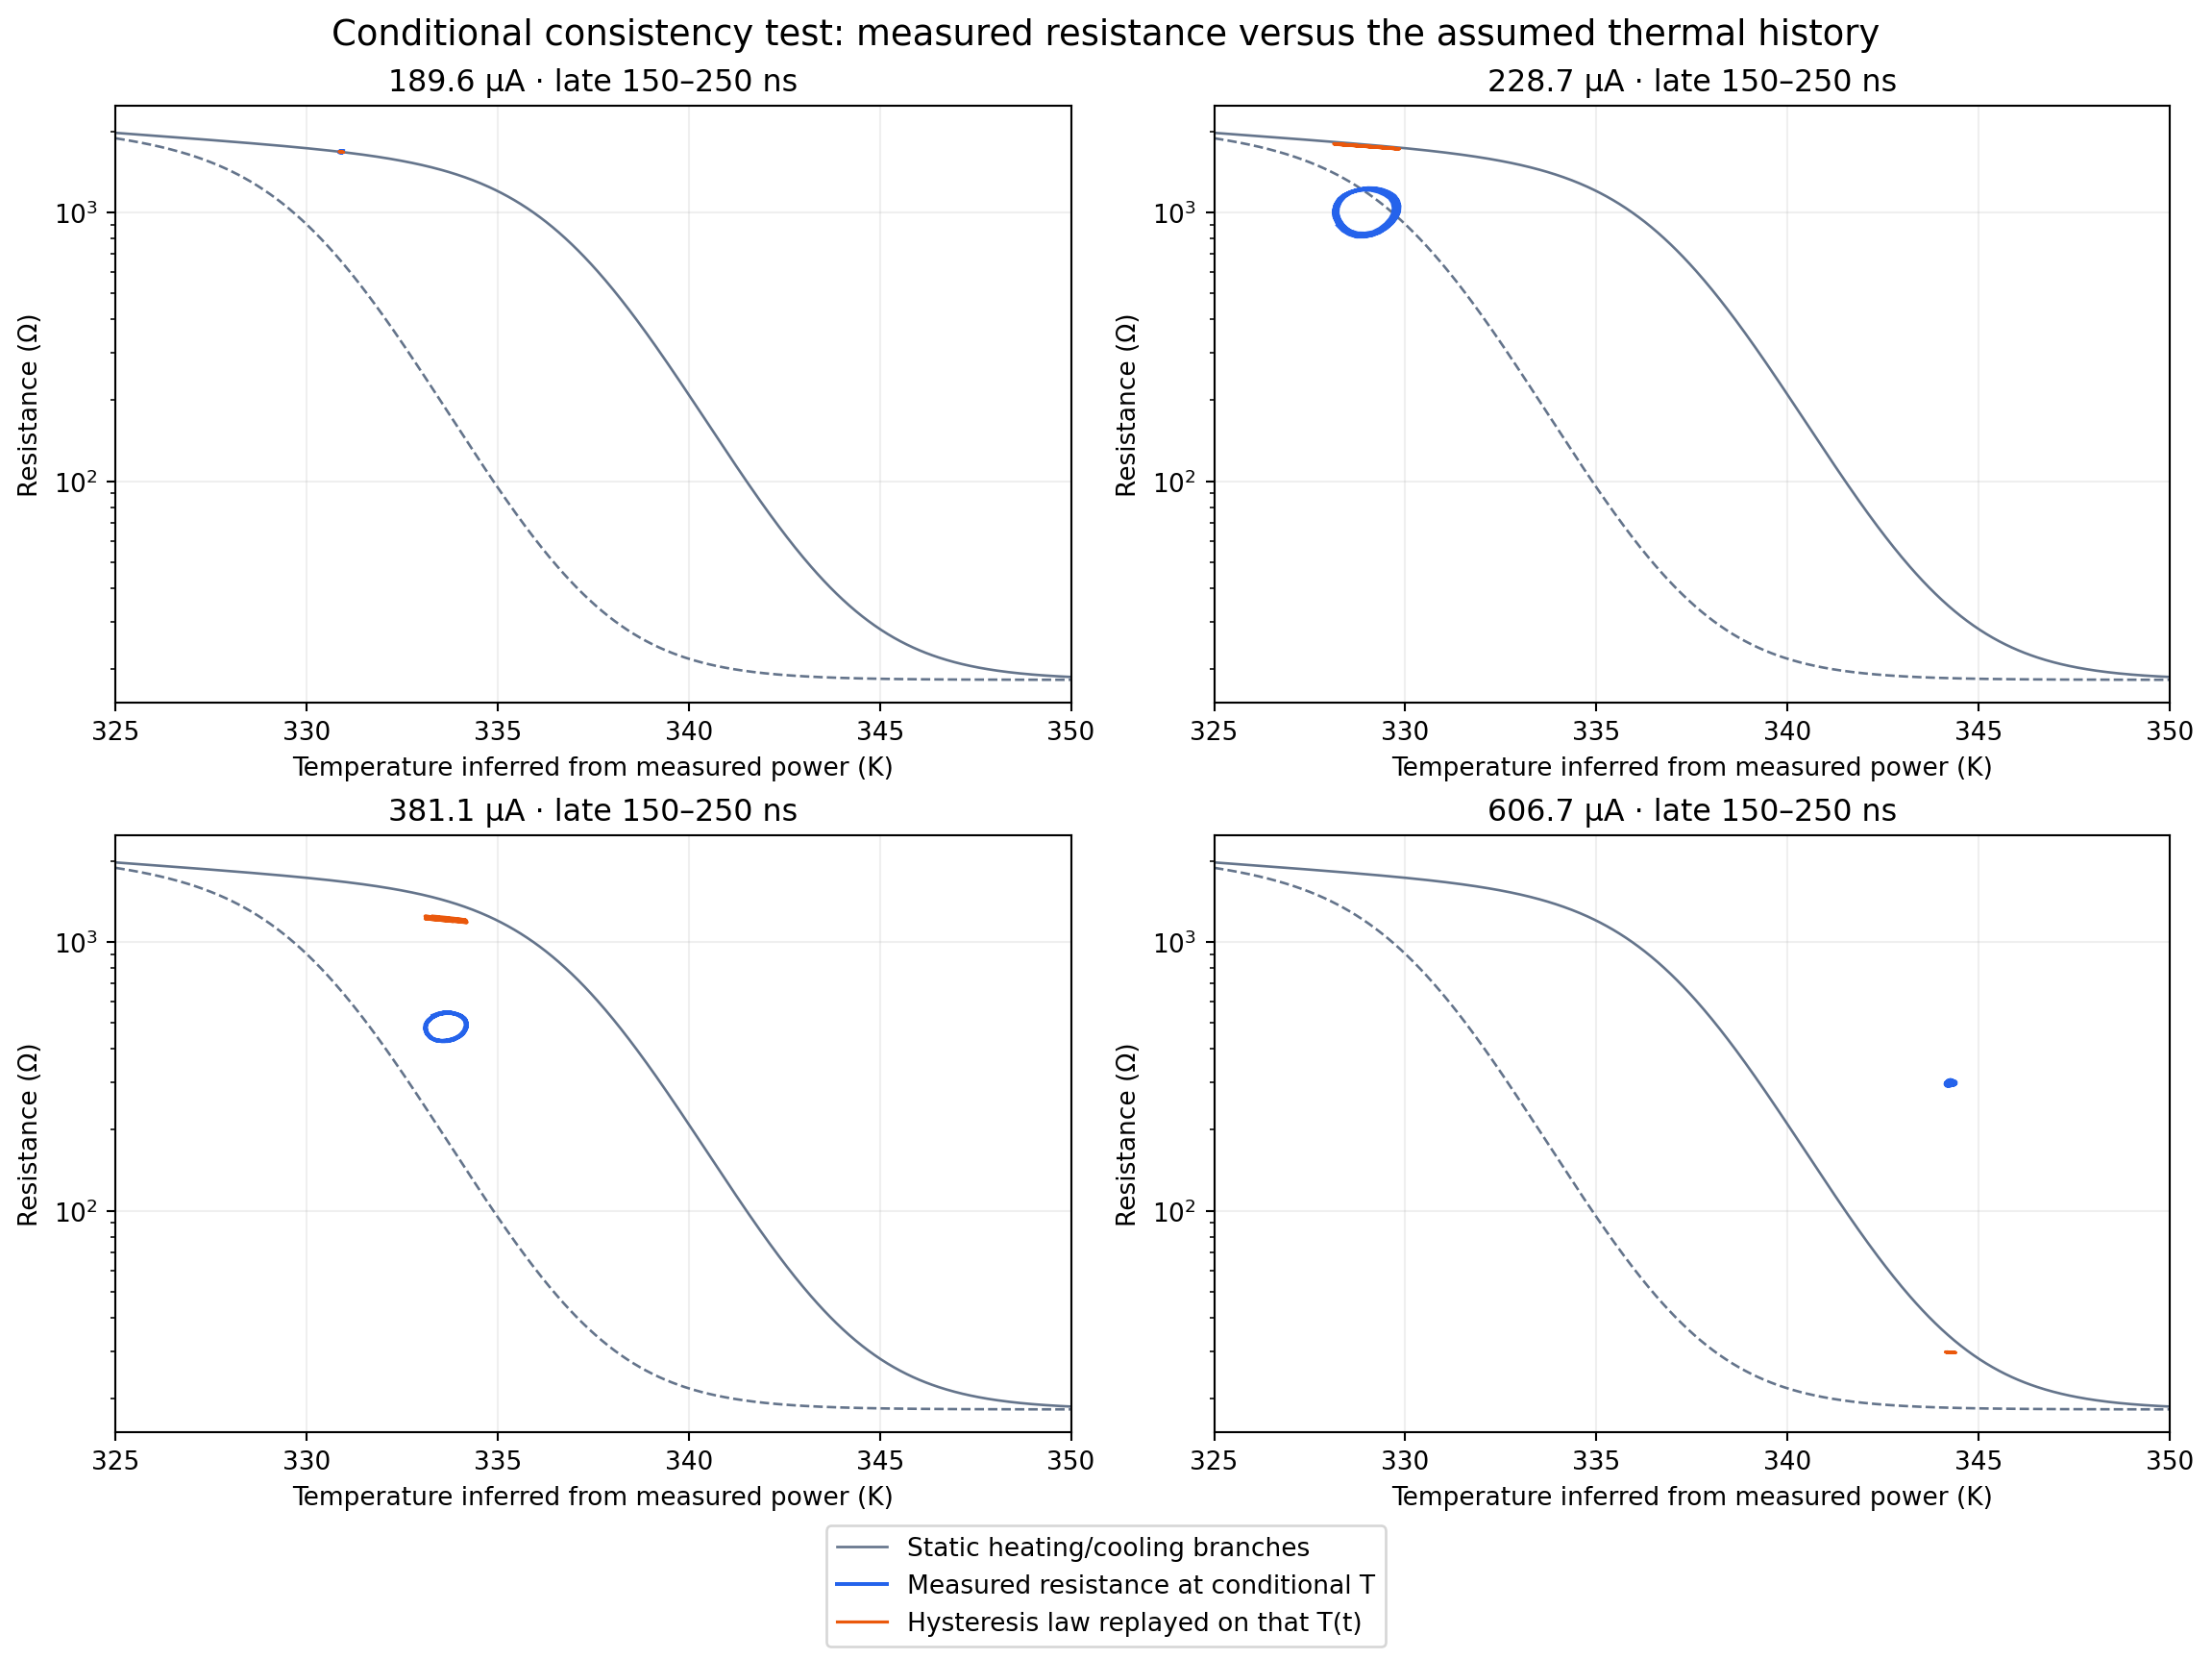
\includegraphics[width=\linewidth]{../public_jobs/20260914_074731_conditional-hysteresis-reconstruction-from-measu_fa4b66/figures/reconstructed_hysteresis.png}
\end{column}
\end{columns}

\slidesource{Bundle \texttt{fa4b66}: scanning \(\gamma=0.157\) to 2.0 did not repair the driven mismatch. A specimen value requires measured minor loops.}
\note{Do not present gamma as fitted. It is inherited from Yuanhang because the available R(T) data contain only a major loop. The later scan shows that changing gamma alone does not explain the discrepancy.}
\end{frame}

% ------------------------------------------------
% Slide 21: environmental conductance
% ------------------------------------------------
\begin{frame}{Environmental Conductance \(S_e\): Use the Last Stable Trace}
\centering

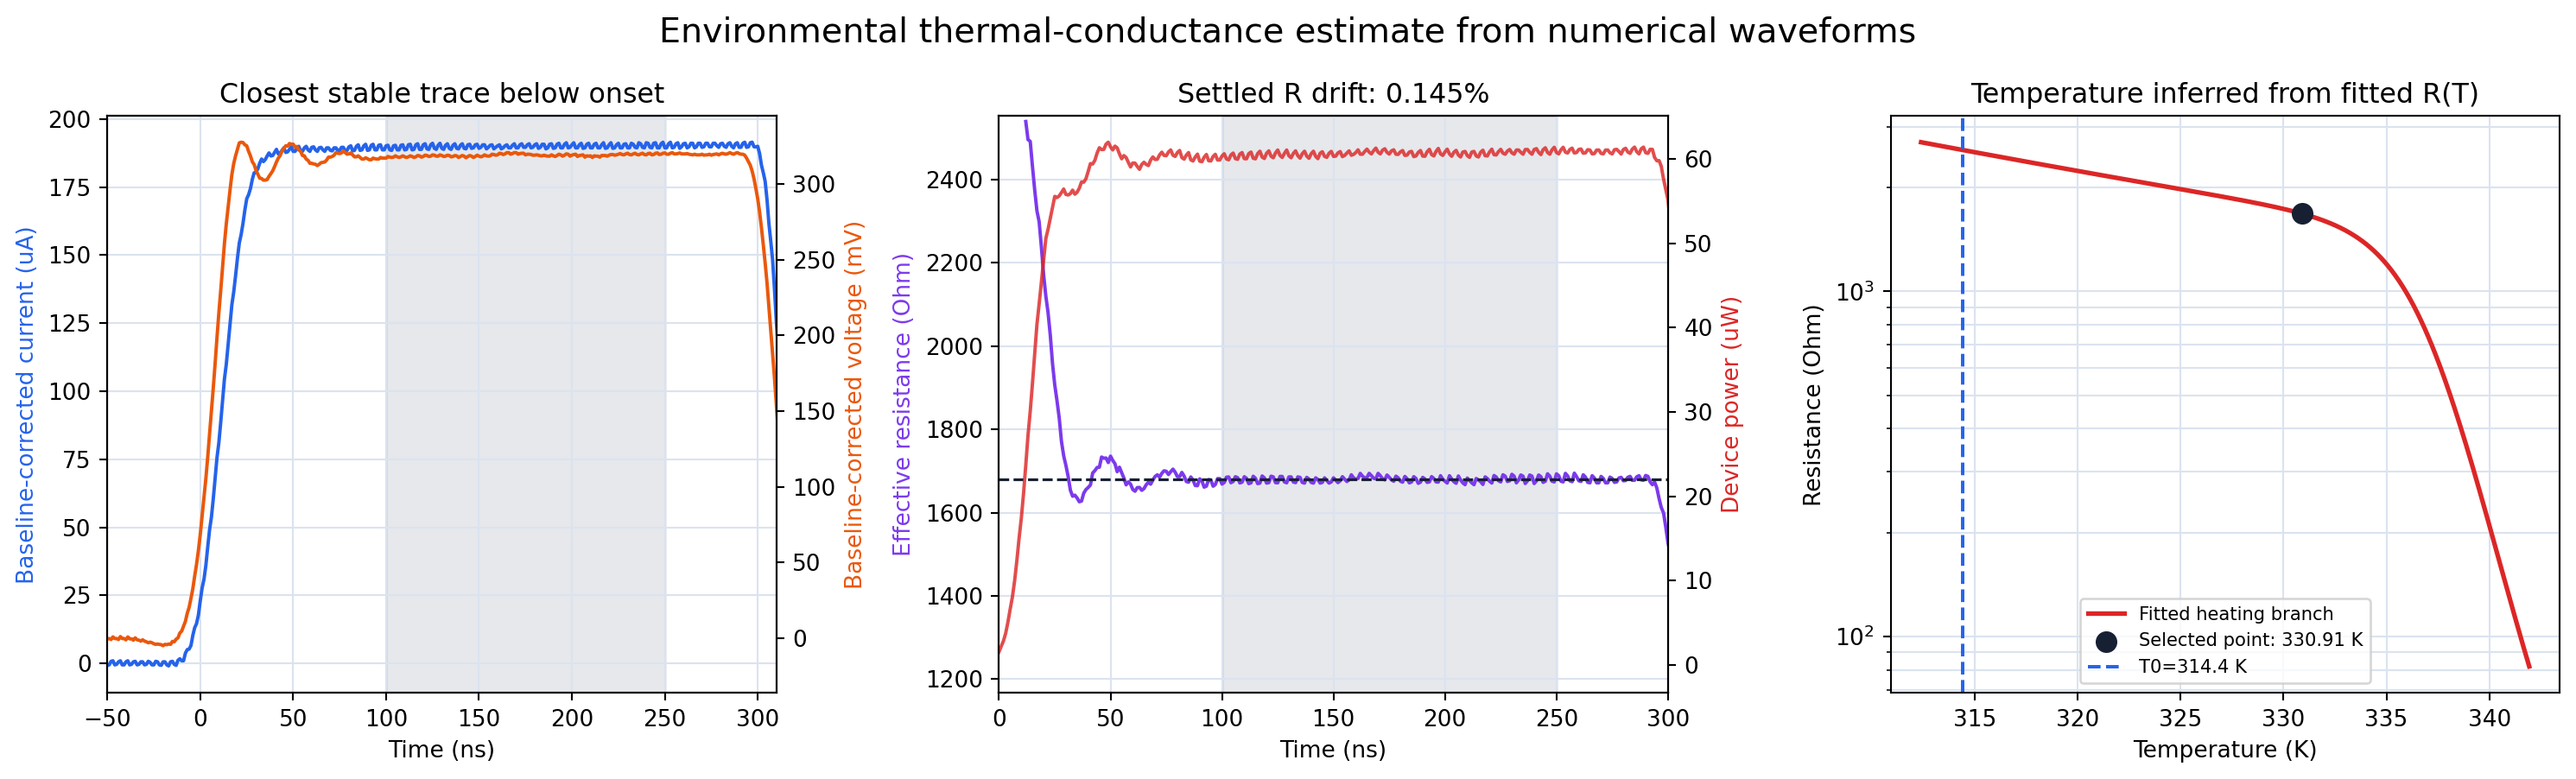
\includegraphics[height=0.55\textheight]{../public_jobs/20260817_153807_environmental-thermal-conductance-estimate_761640/figures/environmental_conductance.png}

\vspace{0.06cm}
\begin{columns}[T,onlytextwidth]
\begin{column}{0.62\textwidth}
\small
At the settled pre-onset point, \(dT/dt\approx0\):
\[
S_e=\frac{P_*}{T_*-T_0}
=\frac{60.658~\mu\mathrm{W}}{330.905-314.4~\mathrm{K}}
\]
\end{column}
\begin{column}{0.35\textwidth}
\begin{alertblock}{Result}
\centering
\(S_e=3.675~\mu\mathrm{W/K}\)\\
\scriptsize conditional range 3.434--4.085 \(\mu\mathrm{W/K}\)
\end{alertblock}
\end{column}
\end{columns}

\slidesource{Selected record: 190.162 \(\mu\)A settled current; resistance drift 0.145\%; reviewed bundle \texttt{761640}.}
\note{The last non-oscillating record maximizes the temperature rise while retaining a quasi-steady balance. The estimate is conditional on interpreting V over I as device resistance and transferring the static heating branch to the driven device.}
\end{frame}

% ------------------------------------------------
% Slide 22: electrical capacitance
% ------------------------------------------------
\begin{frame}{Electrical Capacitance \(C\): A Timing Bound, Not a Detection}

\begin{columns}[T,onlytextwidth]
\begin{column}{0.51\textwidth}
\small
\textbf{Use the complete current balance}
\[
C\frac{dV}{dt}=I_{\mathrm{in}}-\frac{V}{R(T)}
\]

The early, non-switching edges leave no resolved positive capacitive current.
The constrained optimum is \(C=0\). With a 1 ns timing resolution and
\(R(T_0)=2.570~\mathrm{k}\Omega\),
\[
C\lesssim\frac{1~\mathrm{ns}}{2.570~\mathrm{k}\Omega}
=0.39~\mathrm{pF}.
\]

\begin{alertblock}{Adopted modeling value}
\centering
\(\boxed{C=0.39~\mathrm{pF}}\) conservative upper bound
\end{alertblock}
\end{column}

\begin{column}{0.46\textwidth}
\centering
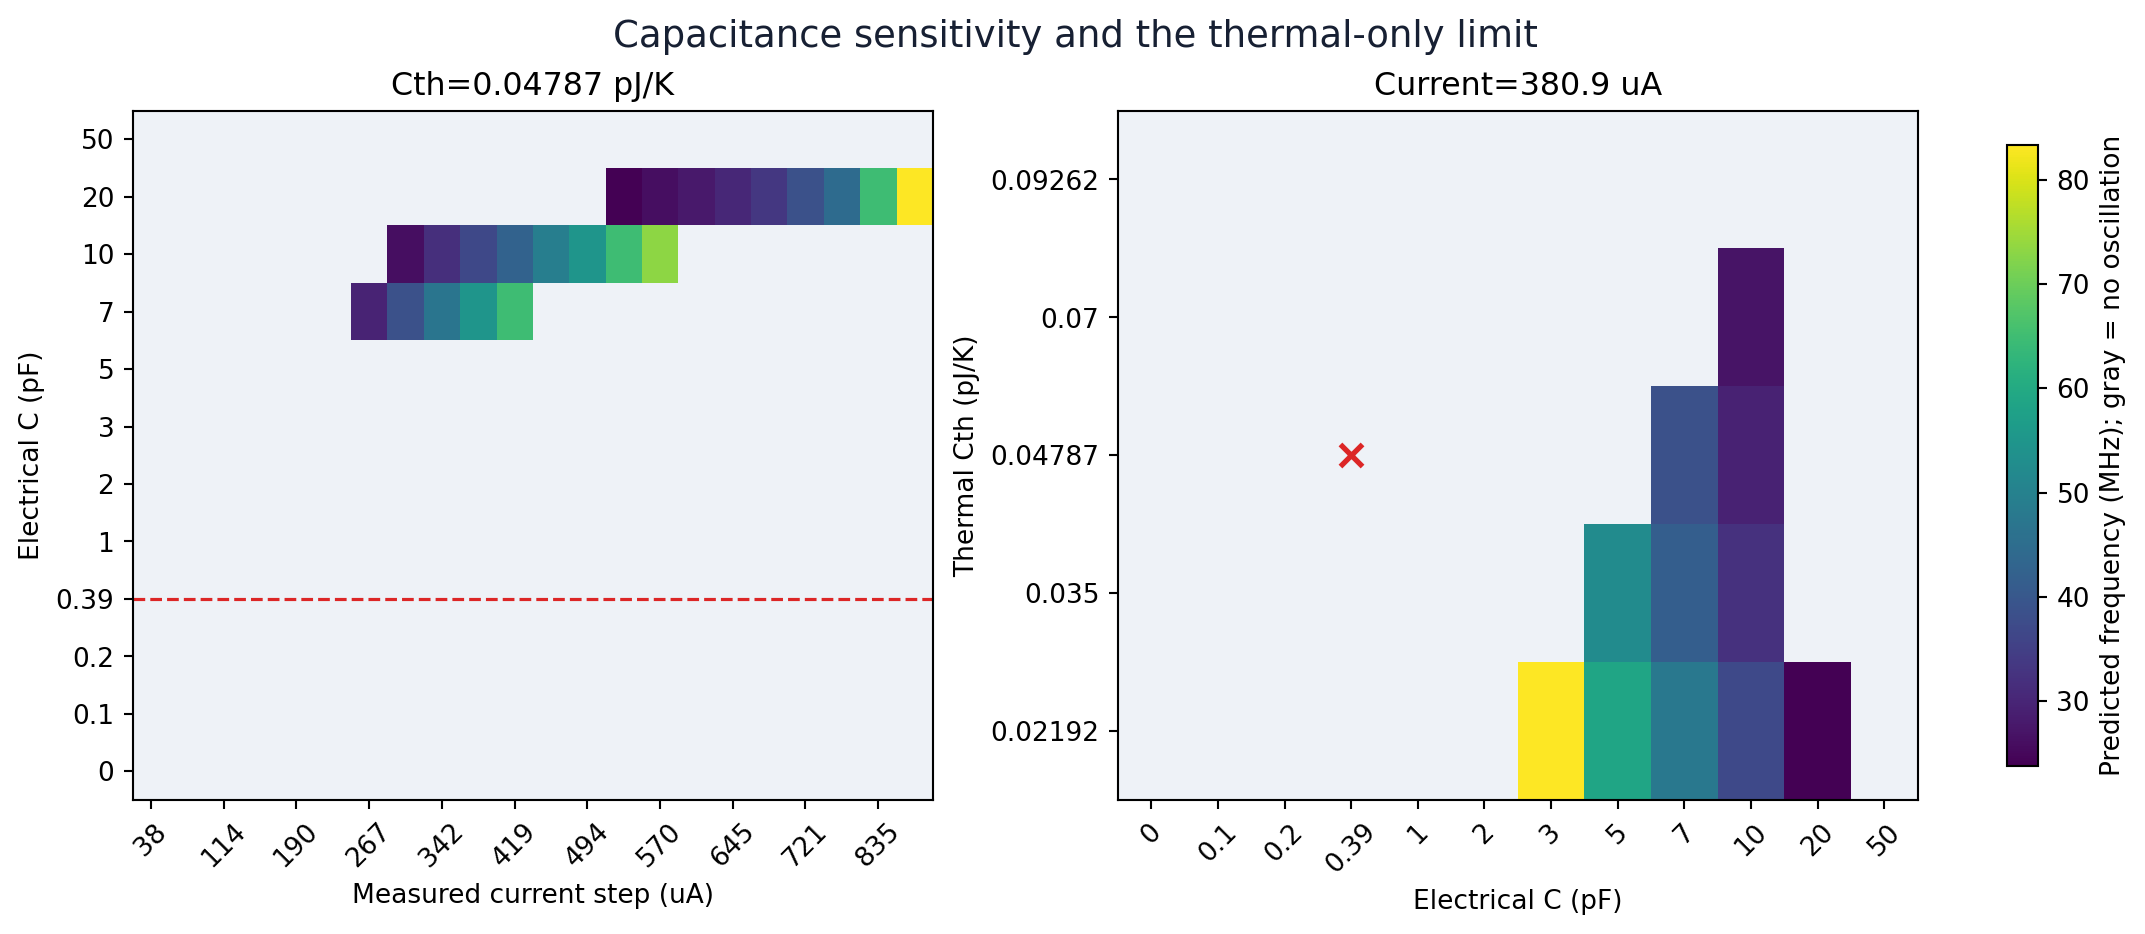
\includegraphics[width=\linewidth]{../public_jobs/20260829_100718_specimen-model-prediction-versus-measured-curren_eefab7/figures/capacitance_sensitivity.png}

\vspace{0.08cm}
\scriptsize
The red dashed line marks 0.39 pF. In the frozen forward study, oscillations
appeared only at several-pF values, outside the timing bound.

\vspace{0.10cm}
\begin{block}{Why 19.8 pF was rejected}
\scriptsize
\(I/(dV/dt)\) neglects the resistive current. It would imply
\(RC=50.9\) ns, a voltage lag absent from the measured edge.
\end{block}
\end{column}
\end{columns}

\slidesource{Electrical-edge analysis and frozen-model sensitivity bundle \texttt{eefab7}.}
\note{The correct conclusion is not that the physical capacitance is exactly zero. The present trace cannot resolve a positive capacitance, so 0.39 pF is an intentionally conservative upper bound.}
\end{frame}

% ------------------------------------------------
% Slide 23: thermal capacitance
% ------------------------------------------------
\begin{frame}{Thermal Capacitance \(C_{th}\): Fit a Shared Heating Time}
\centering

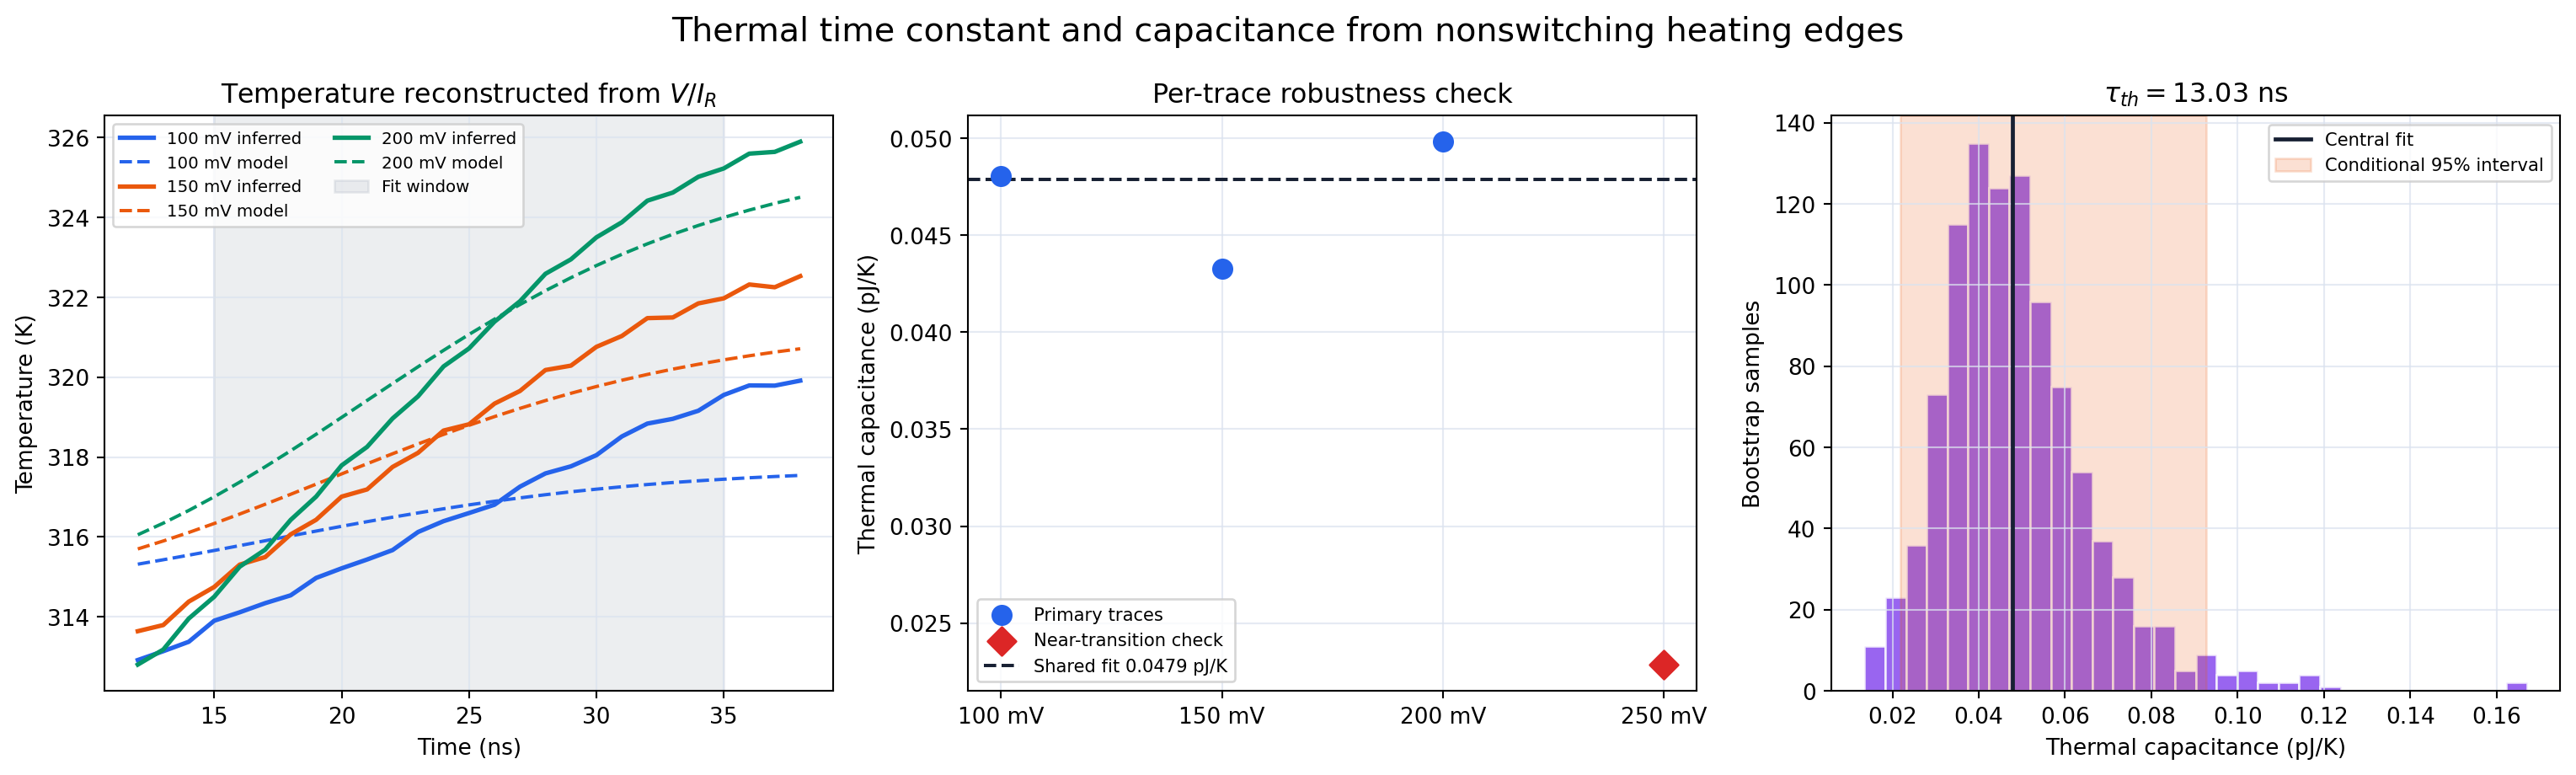
\includegraphics[height=0.48\textheight]{../public_jobs/20260828_112314_thermal-capacitance-estimate-with-conservative-0_aa2469/figures/thermal_capacitance.png}

\vspace{0.05cm}
\begin{columns}[T,onlytextwidth]
\begin{column}{0.62\textwidth}
\scriptsize
\[
I_R=I-C\frac{dV}{dt},\qquad
T_*=R_{\mathrm{heat}}^{-1}\!\left(\frac{V}{I_R}\right),\qquad
C_{th}\frac{dT}{dt}=VI_R-S_e(T-T_0)
\]
One \(C_{th}\) fits the 76.2, 114.2, and 152.2 \(\mu\)A heating edges from
15--35 ns. The 189.6 \(\mu\)A near-transition trace is a sensitivity check.
\end{column}
\begin{column}{0.35\textwidth}
\begin{alertblock}{Result}
\centering
\(C_{th}=0.047873~\mathrm{pJ/K}\)\\[0.08cm]
\(\tau_{th}=C_{th}/S_e=13.026~\mathrm{ns}\)\\[0.08cm]
\scriptsize conditional range 0.021918--0.092624 pJ/K
\end{alertblock}
\end{column}
\end{columns}

\slidesource{Shared transient fit with \(C=0.39\) pF; reviewed bundle \texttt{aa2469}.}
\note{We use the fitted heating branch as a thermometer on moderate non-switching traces, then fit one shared thermal time. The result is conditional on the adopted capacitance bound, conductance, ambient temperature, and a single lumped device temperature.}
\end{frame}

% ------------------------------------------------
% Slide 24: blind validation
% ------------------------------------------------
\begin{frame}{Blind Replay: One Frozen Parameter Set Across All Currents}
\centering

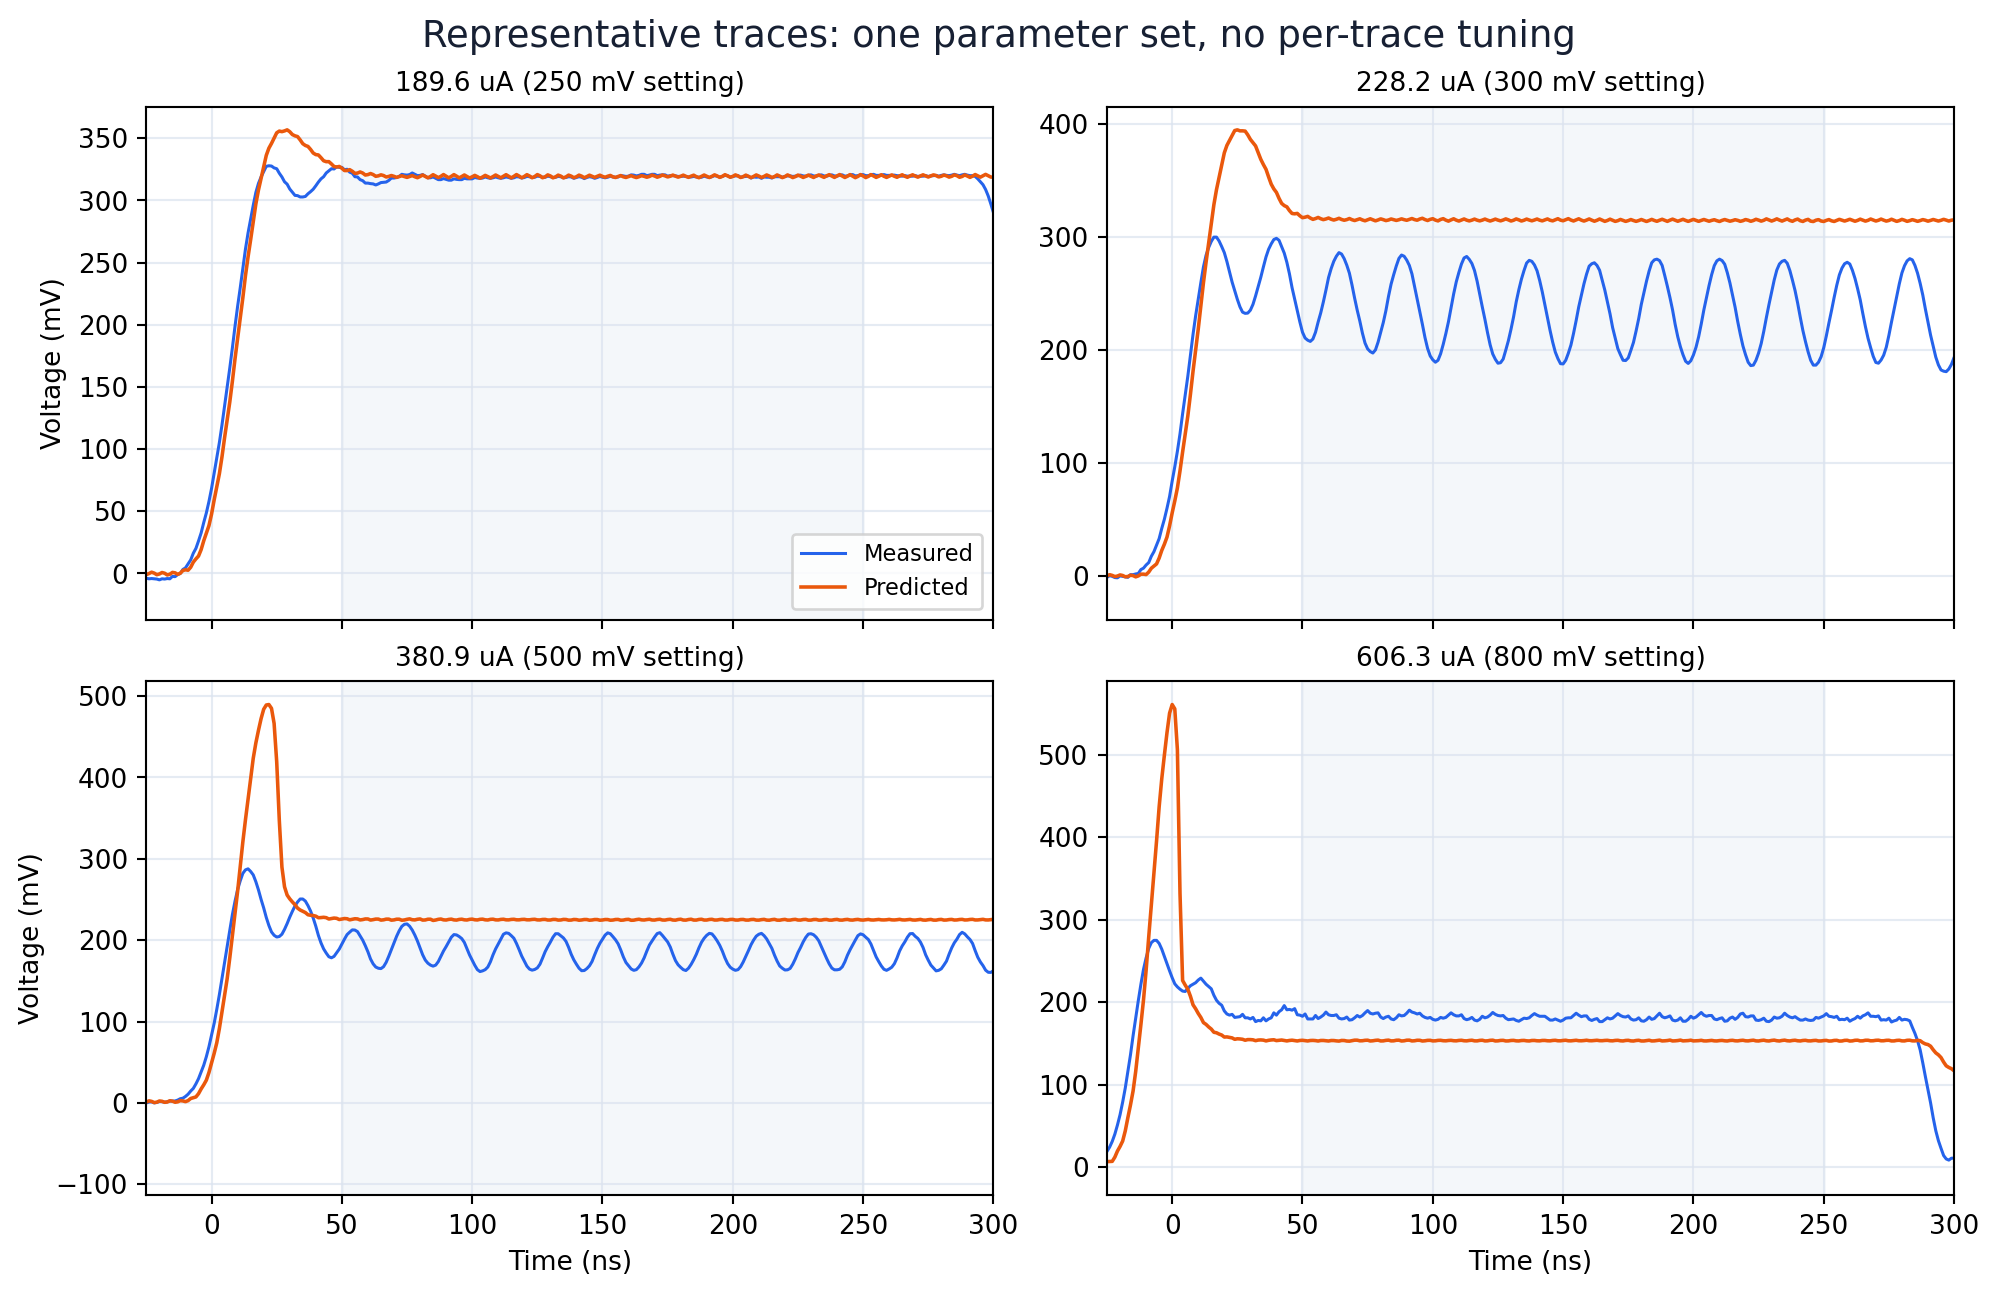
\includegraphics[height=0.56\textheight]{../public_jobs/20260829_100718_specimen-model-prediction-versus-measured-curren_eefab7/figures/representative_traces.png}

\vspace{0.05cm}
\begin{alertblock}{Result}
\scriptsize
The stable 189.6 \(\mu\)A record is reproduced closely. The frozen model predicts
no sustained oscillation in any of the 11 measured oscillatory records and misses
the voltage level at intermediate and high currents.
\end{alertblock}

\slidesource{No per-current tuning; frozen specimen validation bundle \texttt{eefab7}.}
\note{This is the crucial falsification step. The parameter estimates reproduce the pre-onset stable point because that point helped anchor conductance, but the same frozen vector does not reproduce the measured oscillatory region.}
\end{frame}

% ------------------------------------------------
% Slide 25: summary and current status
% ------------------------------------------------
\section{Joint resistance and waveform inference}

\begin{frame}{Can Joint Fitting Rescue the Existing Model?}
\begin{block}{Question}
Can one shared parameter vector explain both the same-device static R(T)
curve and the measured current-driven voltage dynamics?
\end{block}
\begin{columns}[T,onlytextwidth]
\begin{column}{0.49\textwidth}
\textbf{Eleven free quantities}
\begin{itemize}
\item All six major-loop parameters: \(R_0,E_a/k_B,R_m,T_c,w,\beta\).
\item Minor-loop curvature \(\gamma\).
\item \(C,S_e,C_{th},T_0\).
\end{itemize}
\end{column}
\begin{column}{0.49\textwidth}
\textbf{Two controlled searches}
\begin{itemize}
\item Strong static-data penalty: preserve R(T).
\item Weak penalty: diagnostic tradeoff with dynamics.
\item Same waveform loss, bounds and starting population.
\end{itemize}
\end{column}
\end{columns}
\vspace{0.2cm}
\small Nine representative current records train the model; thirteen are excluded
from optimization. All were examined in earlier research, so this is not a new blind test.
\slidesource{Recipe: experiments/current/specimen\_joint\_inference.toml. No change to the physical equations or hysteresis.}
\end{frame}

\begin{frame}{A Bounded Search Across Different Dynamical Regimes}
\begin{enumerate}
\item Normalize the search: log coordinates for positive scales,
\(\tau_{th}=C_{th}/S_e\), and insulating resistance at 315 K instead of \(R_0\).
\item Combine historical fits, nearby perturbations and a space-filling sample;
reject severe static-data disagreement before running the simulator.
\item Run differential evolution with 24 candidates and three generations per
objective, then at most 24 Powell evaluations per objective.
\item Cache repeated simulations; verify the winners and historical references
on all 22 currents at 0.025, 0.0125 and 0.00625 ns.
\end{enumerate}
\begin{alertblock}{Budget, not a global optimum}
At most 240 objective calls. A short search can find an improvement;
failure to fit does not prove that no parameter vector exists.
\end{alertblock}
\slidesource{Search timestep: 0.05 ns. Full recorded pre-pulse history retained; unused post-250 ns tail omitted.}
\end{frame}

\begin{frame}{Fit Persistent Features Alongside the Static Curve}
\[
L=L_{\rm mean}+3L_{\rm periodic\ amplitude}+L_{\rm robust\ amplitude}
+0.5L_f+\lambda_R\left(\frac{\mathrm{RMSE}_{\log_{10}R}}{0.05}\right)^2.
\]
\begin{itemize}
\item Compare amplitude and mean in four 50 ns windows, from 50 to 250 ns.
\item Amplitude uses log ratios with a 3 mV floor; mean-voltage scale is 20 mV.
\item Frequency uses a 10 MHz scale and a smooth amplitude/coherence gate;
missing cycles are still penalized by their amplitude error.
\item \(\lambda_R=4\) preserves the static curve; \(\lambda_R=0.15\) explores
the cost of allowing it to move. Both reject static RMSE above 0.35 decades.
\end{itemize}
\begin{block}{Separate acceptance check}
Report late mean, amplitude, frequency and four-window persistence independently.
Loss weights are engineering choices, not experimental confidence intervals.
\end{block}
\end{frame}

% Joint-fit result frames are included from a run-specific generated source.
% Numerical source: immutable joint-fit bundle 6b5d8f, 21 September 2026.
\newcommand{\jointbundle}{../public_jobs/20260921_130032_budgeted-joint-resistance-and-waveform-inference_6b5d8f}

\begin{frame}{Joint Fitting Improves a Score, but Not Every Requirement}
\centering
\small
\begin{tabular}{lrrrr}
\toprule
Shared candidate & Static RMSE & Mean RMSE & Amplitude MAE & Recovered \\
 & (decades) & (mV) & (mV) & /11 \\
\midrule
Frozen estimates & 0.0366 & 45.3 & 44.3 & 0 \\
Prior anchored, replayed & 0.0426 & 50.9 & 140.1 & 9 \\
Joint: static-preserving & 0.0495 & 50.5 & 62.0 & 4 \\
Joint: dynamic diagnostic & 0.1433 & 60.2 & 90.3 & 5 \\
\bottomrule
\end{tabular}
\vspace{0.3cm}
\begin{block}{Useful improvement}
The static-preserving fit reduces the validation feature score from 15.16
(prior anchored) to 10.07: a 33.5\% improvement on the thirteen excluded currents.
\end{block}
\begin{alertblock}{Unresolved tradeoff}
Smaller amplitude errors come with fewer sustained oscillators. Mean voltage
does not improve over the frozen baseline. No new physical calibration is adopted.
\end{alertblock}
\slidesource{0.00625 ns. Mean error: 22 records. Periodic-amplitude error: the same 11 measured oscillators. Zero false positives. Bundle 6b5d8f.}
\end{frame}

\begin{frame}{Static Resistance and Dynamic Waveforms Compete}
\centering

\includegraphics[width=\textwidth]{\jointbundle/figures/joint_summary.png}
\begin{block}{Interpretation}
Allowing all resistance parameters to move is not enough, within this budget,
to match static R(T), the output plateau and the full oscillation window together.
\end{block}
\slidesource{Plots use one parameter vector per candidate and all 22 records. Horizontal source settings identify records; the simulated input is the measured current waveform.}
\end{frame}

\begin{frame}{Representative Waveforms: The Remaining Failures Are Visible}
\centering

\includegraphics[height=0.77\textheight]{\jointbundle/figures/joint_traces.png}
\slidesource{0.00625 ns; no per-current fitting or phase alignment. Settings 250/300/500/800 mV identify measured current steps near 190/228/381/606 microampere.}
\end{frame}

\begin{frame}{What the Optimizer Changed}
\begin{columns}[T,onlytextwidth]
\begin{column}{0.62\textwidth}
\scriptsize
\begin{tabular}{lrrr}
\toprule
Parameter & Frozen & Static-preserving & Diagnostic \\
\midrule
\(R_0\) (\(\Omega\)) & 0.7989 & 0.6893 & 0.8620 \\
\(E_a/k_B\) (K) & 2537.0 & 2575.1 & 2485.1 \\
\(R_m\) (\(\Omega\)) & 18.22 & 20.06 & 17.57 \\
\(T_c\) (K) & 333.49 & 333.31 & 332.18 \\
\(w\) (K) & 6.882 & 6.371 & 7.243 \\
\(\beta\) (K\(^{-1}\)) & 0.2992 & 0.2800 & 0.3639 \\
\(\gamma\) & 0.9563 & 0.1757 & 0.1787 \\
\(T_0\) (K) & 314.40 & 314.53 & 313.90 \\
\(C\) (pF) & 0.390 & 6.806 & 4.964 \\
\(S_e\) (\(\mu\)W/K) & 3.675 & 3.738 & 3.519 \\
\(C_{th}\) (pJ/K) & 0.04787 & 0.05928 & 0.03970 \\
\(\tau_{th}\) (ns), derived & 13.03 & 15.86 & 11.28 \\
\bottomrule
\end{tabular}
\end{column}
\begin{column}{0.35\textwidth}
\begin{block}{Recurring conflict}
\small Both fits favor electrical capacitance well above the conditional
0.39 pF timing bound and a much smaller minor-loop parameter.
\end{block}
\begin{alertblock}{Effective values}
\small These values minimize the chosen objective. They are not independent
measurements of device capacitance, heat capacity or filament properties.
\end{alertblock}
\end{column}
\end{columns}
\slidesource{All six major-loop quantities were free; numerical values from parameters.csv. Same-device identity was confirmed by Gabriel.}
\end{frame}

\begin{frame}{Verification and the Decision After This Search}
\footnotesize
\begin{tabular}{lrr}
\toprule
Last refinement: 0.0125 to 0.00625 ns & Static-preserving & Diagnostic \\
\midrule
Maximum late-mean change, all currents & 0.34 mV & 4.04 mV \\
Maximum periodic-amplitude change, persistent records & 2.52\% & 1.95\% \\
Maximum frequency change, persistent records & 0.16\% & 0.44\% \\
Persistent records at both fine steps & 4 & 5 \\
\bottomrule
\end{tabular}
\vspace{0.15cm}
\begin{itemize}
\item 240 objective calls, 214 unique candidates, 201 search simulations;
search wall time 153 s on this machine. Both optimizers exhausted their caps.
\item Static-preserving search loss improved 15.1\% over its best starting
candidate; diagnostic search loss improved 18.7\%. These are coarse-search scores.
\item Final selection must use fine-step feature errors \emph{and} persistence.
No candidate meets the complete experimental target.
\end{itemize}
\begin{block}{Next decision}
Preserve these candidates as tradeoff evidence. Calibrate the TIA/device boundary
and driven switching law before treating a more flexible fit as physical truth.
\end{block}
\slidesource{Amplitude/frequency changes use records persistent at both fine steps. Full verification: all 22 records at three steps.}
\end{frame}

\begin{frame}{Expanded Search: Better Mean Voltage, Remaining Tradeoffs}
\small
\(T_0\) was already free over 308--322 K. Added persistence penalties,
previous joint-fit seeds and a larger DE/Powell budget; search step halved to 0.025 ns.
\vspace{0.2cm}
\scriptsize
\begin{tabular}{lrrrr}
\toprule
Candidate & Static log RMSE & Mean error (mV) & Recovered / 11 & Amplitude error (mV)\\
\midrule
Prior anchored & 0.0426 & 50.9 & 9 & 140.1\\
Prior joint, stronger static & 0.0495 & 50.5 & 4 & 62.0\\
Expanded, stronger static & 0.0489 & 44.6 & 7 & 127.9\\
Expanded, relaxed static & 0.1473 & 39.8 & 6 & 130.6\\
\bottomrule
\end{tabular}
\vspace{0.2cm}
\begin{itemize}
\item 456 objective calls; 400 unique candidates; 399 search simulations; 673 s.
\item Stronger-static candidate: \(T_0=313.09\) K, \(C=4.650\) pF;
relaxed candidate: \(T_0=315.00\) K, \(C=12.334\) pF. Neither hits the ambient bounds.
\item Stronger-static recall falls from 8 to 7 at the finest timestep.
No candidate resolves the voltage, amplitude and persistence mismatch together.
\end{itemize}
\slidesource{Bundle 694804. All results at 0.00625 ns; mean-voltage RMSE on 22 records, periodic-amplitude MAE on the same 11 measured oscillators. New loss; historical vectors re-evaluated.}
\end{frame}

\begin{frame}{Editable Laboratory: Compare Every Measured Current}
\begin{columns}[T,onlytextwidth]
\begin{column}{0.49\textwidth}
\begin{block}{Edit and replay}
\small Load original or fitted parameters. Edit the resistance law separately
from capacitance, heat capacity, thermal conductance and ambient temperature.
Press \textbf{Run all measured currents} to use one shared parameter vector.
\end{block}
\begin{block}{Inspect}
\small Voltage overlays compare experiment and simulation. A second plot shows
simulated resistance versus time. The bottom slider selects the current;
optional GIFs animate a time cursor over both plots.
\end{block}
\end{column}
\begin{column}{0.48\textwidth}
\begin{block}{Reproduce}
\small Each run saves numerical traces, metrics, a standalone HTML current
slider, per-current GIFs and a parameter recipe. Completed runs are preserved.
\end{block}
\begin{alertblock}{Interpretation}
\small Manual replay is exploratory. Check smaller timesteps before interpreting
an improved fit. Exported voltage still needs circuit calibration; simulated
resistance is not a measured voltage/current ratio.
\end{alertblock}
\end{column}
\end{columns}
\vspace{0.2cm}
\small Start with \texttt{neuristor playground}; open \texttt{127.0.0.1:8502}.
\slidesource{Workflow: replay-lab. Recipe: experiments/current/specimen\_lab\_replay.toml. Expanded-search notes: docs/EXPANDED\_SEARCH\_20260922.md.}
\end{frame}


\begin{frame}{Frozen Baseline and What the Joint Fit Tests}

\begin{columns}[T,onlytextwidth]
\begin{column}{0.50\textwidth}
\scriptsize
\begin{tabular}{@{}lll@{}}
\toprule
\textbf{Quantity} & \textbf{Value} & \textbf{Evidence status} \\
\midrule
\(I(t)\) & measured waveform & direct input \\
\(T_0\) & 314.4 K & adopted condition \\
\(R_m\) & 18.215 \(\Omega\) & major-loop fit \\
\(T_c\) & 333.494 K & major-loop fit \\
\(w\) & 6.882 K & major-loop fit \\
\(\beta\) & 0.2992 K\(^{-1}\) & major-loop fit \\
\(\gamma\) & 0.95627 & borrowed value \\
\(S_e\) & 3.675 \(\mu\)W/K & conditional estimate \\
\(C\) & 0.39 pF & upper bound \\
\(C_{th}\) & 0.047873 pJ/K & conditional fit \\
\(\tau_{th}\) & 13.026 ns & derived \\
\bottomrule
\end{tabular}
\end{column}

\begin{column}{0.46\textwidth}
\begin{block}{What the work established}
\small
The mechanism implementation works, the static resistance loop is tightly fit,
and every dynamic parameter now has an explicit evidence trail.
\end{block}

\begin{alertblock}{What the mismatch tells us}
\small
The joint search tests whether coupled parameter changes reduce the discrepancy.
Physical interpretation still requires the actual VO\textsubscript{2} terminal
voltage and branch current, driven minor loops, and an independent thermal response.
\end{alertblock}
\end{column}
\end{columns}

\vspace{0.18cm}
\begin{center}
\Large Thank you
\end{center}

\note{End with the distinction between a documented parameter estimate and a successful predictive model. The mismatch is scientifically useful because it identifies the measurement boundary and driven device state as the next measurements to resolve.}
\end{frame}

% ------------------------------------------------
% Backup slides
% ------------------------------------------------
\appendix

\begin{frame}{Backup: Representative Timestep Convergence}
\centering

\begin{tabular}{rrr}
\toprule
\(\Delta t\) (ns) & Period (ns) & Frequency (MHz) \\
\midrule
0.015820 & 123.206 & 8.116 \\
0.007910 & 123.135 & 8.121 \\
0.003955 & 123.095 & 8.124 \\
\bottomrule
\end{tabular}

\vspace{0.45cm}

\begin{block}{Interpretation}
The period approaches a stable value as the timestep is halved. This is the
expected signature of a physical solution being resolved more accurately, rather
than an oscillation created by the numerical grid.
\end{block}

\slidesource{Representative Yuanhang current-source case: \(I=\SI{1640.226}{\micro\ampere}\).}
\end{frame}

\begin{frame}{Backup: Final Current-Source Standard}

\[
\boxed{
\begin{aligned}
C\frac{dV}{dt} &= I_{in}-\frac{V}{R},\\
C_{th}\frac{dT}{dt} &= \frac{V^2}{R}-S_e(T-T_0),\\
R(T,\mathcal H) &= R_m+R_0e^{(E_a/k_B)/T}g(T,\mathcal H).
\end{aligned}
}
\]

\begin{itemize}
    \item Exactly one VO\textsubscript{2} device/domain and one thermal node.
    \item Upstream-faithful Yuanhang/Almeida hysteresis and reversal memory.
    \item Deterministic default \(\sigma=0\); optional stochastic heating remains available.
    \item Obsolete delayed-phase, double-thermal, and multidomain variants are not active models.
\end{itemize}
\end{frame}

\begin{frame}{Backup: Reproducibility Trail}

\begin{itemize}
    \item Fitted sample: \texttt{100425 chip1 gap3}.
    \item Major-loop fit: \texttt{0849a9}; conductance estimate: \texttt{761640}.
    \item Thermal-capacitance fit: \texttt{aa2469}; frozen validation: \texttt{eefab7}.
    \item Each reviewed bundle stores resolved inputs, metrics, numerical tables, figures, and a human-readable report.
    \item Regression tests cover voltage and current models, hysteresis fidelity, convergence, analysis workflows, and archive validation.
\end{itemize}

\begin{block}{AI-use principle}
Codex was allowed to automate implementation and search, but successful results
were accepted only after model-preservation, physical interpretation, and
numerical-convergence checks.
\end{block}
\end{frame}

\end{document}
